
%% bare_jrnl.tex
%% V1.4a
%% 2014/09/17
%% by Michael Shell
%% see http://www.michaelshell.org/
%% for current contact information.
%%
%% This is a skeleton file demonstrating the use of IEEEtran.cls
%% (requires IEEEtran.cls version 1.8a or later) with an IEEE
%% journal paper.
%%
%% Support sites:
%% http://www.michaelshell.org/tex/ieeetran/
%% http://www.ctan.org/tex-archive/macros/latex/contrib/IEEEtran/
%% and
%% http://www.ieee.org/

%%*************************************************************************
%% Legal Notice:
%% This code is offered as-is without any warranty either expressed or
%% implied; without even the implied warranty of MERCHANTABILITY or
%% FITNESS FOR A PARTICULAR PURPOSE! 
%% User assumes all risk.
%% In no event shall IEEE or any contributor to this code be liable for
%% any damages or losses, including, but not limited to, incidental,
%% consequential, or any other damages, resulting from the use or misuse
%% of any information contained here.
%%
%% All comments are the opinions of their respective authors and are not
%% necessarily endorsed by the IEEE.
%%
%% This work is distributed under the LaTeX Project Public License (LPPL)
%% ( http://www.latex-project.org/ ) version 1.3, and may be freely used,
%% distributed and modified. A copy of the LPPL, version 1.3, is included
%% in the base LaTeX documentation of all distributions of LaTeX released
%% 2003/12/01 or later.
%% Retain all contribution notices and credits.
%% ** Modified files should be clearly indicated as such, including  **
%% ** renaming them and changing author support contact information. **
%%
%% File list of work: IEEEtran.cls, IEEEtran_HOWTO.pdf, bare_adv.tex,
%%                    bare_conf.tex, bare_jrnl.tex, bare_conf_compsoc.tex,
%%                    bare_jrnl_compsoc.tex, bare_jrnl_transmag.tex
%%*************************************************************************


% *** Authors should verify (and, if needed, correct) their LaTeX system  ***
% *** with the testflow diagnostic prior to trusting their LaTeX platform ***
% *** with production work. IEEE's font choices and paper sizes can       ***
% *** trigger bugs that do not appear when using other class files.       ***                          ***
% The testflow support page is at:
% http://www.michaelshell.org/tex/testflow/



\documentclass[a4paper,conference]{IEEEtran}
%\documentclass[a4paper,journal]{IEEEtran}
%\documentclass[a4paper,draftcls,onecolumn]{IEEEtran}
%
% If IEEEtran.cls has not been installed into the LaTeX system files,
% manually specify the path to it like:
% \documentclass[journal]{../sty/IEEEtran}

% Some very useful LaTeX packages include:
% (uncomment the ones you want to load)


% *** MISC UTILITY PACKAGES ***
%
%\usepackage{ifpdf}
% Heiko Oberdiek's ifpdf.sty is very useful if you need conditional
% compilation based on whether the output is pdf or dvi.
% usage:
% \ifpdf
%   % pdf code
% \else
%   % dvi code
% \fi
% The latest version of ifpdf.sty can be obtained from:
% http://www.ctan.org/tex-archive/macros/latex/contrib/oberdiek/
% Also, note that IEEEtran.cls V1.7 and later provides a builtin
% \ifCLASSINFOpdf conditional that works the same way.
% When switching from latex to pdflatex and vice-versa, the compiler may
% have to be run twice to clear warning/error messages.

% *** CITATION PACKAGES ***
%
\usepackage{cite}
% cite.sty was written by Donald Arseneau
% V1.6 and later of IEEEtran pre-defines the format of the cite.sty package
% \cite{} output to follow that of IEEE. Loading the cite package will
% result in citation numbers being automatically sorted and properly
% "compressed/ranged". e.g., [1], [9], [2], [7], [5], [6] without using
% cite.sty will become [1], [2], [5]--[7], [9] using cite.sty. cite.sty's
% \cite will automatically add leading space, if needed. Use cite.sty's
% noadjust option (cite.sty V3.8 and later) if you want to turn this off
% such as if a citation ever needs to be enclosed in parenthesis.
% cite.sty is already installed on most LaTeX systems. Be sure and use
% version 5.0 (2009-03-20) and later if using hyperref.sty.
% The latest version can be obtained at:
% http://www.ctan.org/tex-archive/macros/latex/contrib/cite/
% The documentation is contained in the cite.sty file itself.


% *** GRAPHICS RELATED PACKAGES ***
%
\ifCLASSINFOpdf
	 \usepackage[pdftex]{graphicx}
	 % declare the path(s) where your graphic files are
	 % \graphicspath{{../pdf/}{../jpeg/}}
	 \graphicspath{{media/}}
	 % and their extensions so you won't have to specify these with
	 % every instance of \includegraphics
	 \DeclareGraphicsExtensions{.pdf,.jpeg,.png,.jpg,.eps}
\else
% or other class option (dvipsone, dvipdf, if not using dvips). graphicx
% will default to the driver specified in the system graphics.cfg if no
% driver is specified.
% \usepackage[dvips]{graphicx}
% declare the path(s) where your graphic files are
% \graphicspath{{../eps/}}
% and their extensions so you won't have to specify these with
% every instance of \includegraphics
% \DeclareGraphicsExtensions{.eps}
\fi
% graphicx was written by David Carlisle and Sebastian Rahtz. It is
% required if you want graphics, photos, etc. graphicx.sty is already
% installed on most LaTeX systems. The latest version and documentation
% can be obtained at: 
% http://www.ctan.org/tex-archive/macros/latex/required/graphics/
% Another good source of documentation is "Using Imported Graphics in
% LaTeX2e" by Keith Reckdahl which can be found at:
% http://www.ctan.org/tex-archive/info/epslatex/
%
% latex, and pdflatex in dvi mode, support graphics in encapsulated
% postscript (.eps) format. pdflatex in pdf mode supports graphics
% in .pdf, .jpeg, .png and .mps (metapost) formats. Users should ensure
% that all non-photo figures use a vector format (.eps, .pdf, .mps) and
% not a bitmapped formats (.jpeg, .png). IEEE frowns on bitmapped formats
% which can result in "jaggedy"/blurry rendering of lines and letters as
% well as large increases in file sizes.
%
% You can find documentation about the pdfTeX application at:
% http://www.tug.org/applications/pdftex


% *** MATH PACKAGES ***
%
\usepackage[cmex10]{amsmath}
\usepackage{amssymb}
% A popular package from the American Mathematical Society that provides
% many useful and powerful commands for dealing with mathematics. If using
% it, be sure to load this package with the cmex10 option to ensure that
% only type 1 fonts will utilized at all point sizes. Without this option,
% it is possible that some math symbols, particularly those within
% footnotes, will be rendered in bitmap form which will result in a
% document that can not be IEEE Xplore compliant!
%
% Also, note that the amsmath package sets \interdisplaylinepenalty to 10000
% thus preventing page breaks from occurring within multiline equations. Use:
%\interdisplaylinepenalty=2500
% after loading amsmath to restore such page breaks as IEEEtran.cls normally
% does. amsmath.sty is already installed on most LaTeX systems. The latest
% version and documentation can be obtained at:
% http://www.ctan.org/tex-archive/macros/latex/required/amslatex/math/


% *** SPECIALIZED LIST PACKAGES ***
%
%\usepackage{algorithmic}
% algorithmic.sty was written by Peter Williams and Rogerio Brito.
% This package provides an algorithmic environment fo describing algorithms.
% You can use the algorithmic environment in-text or within a figure
% environment to provide for a floating algorithm. Do NOT use the algorithm
% floating environment provided by algorithm.sty (by the same authors) or
% algorithm2e.sty (by Christophe Fiorio) as IEEE does not use dedicated
% algorithm float types and packages that provide these will not provide
% correct IEEE style captions. The latest version and documentation of
% algorithmic.sty can be obtained at:
% http://www.ctan.org/tex-archive/macros/latex/contrib/algorithms/
% There is also a support site at:
% http://algorithms.berlios.de/index.html
% Also of interest may be the (relatively newer and more customizable)
% algorithmicx.sty package by Szasz Janos:
% http://www.ctan.org/tex-archive/macros/latex/contrib/algorithmicx/


% *** ALIGNMENT PACKAGES ***
%
%\usepackage{array}
% Frank Mittelbach's and David Carlisle's array.sty patches and improves
% the standard LaTeX2e array and tabular environments to provide better
% appearance and additional user controls. As the default LaTeX2e table
% generation code is lacking to the point of almost being broken with
% respect to the quality of the end results, all users are strongly
% advised to use an enhanced (at the very least that provided by array.sty)
% set of table tools. array.sty is already installed on most systems. The
% latest version and documentation can be obtained at:
% http://www.ctan.org/tex-archive/macros/latex/required/tools/


% IEEEtran contains the IEEEeqnarray family of commands that can be used to
% generate multiline equations as well as matrices, tables, etc., of high
% quality.


% *** SUBFIGURE PACKAGES ***
\ifCLASSOPTIONcompsoc
	\usepackage[caption=false,font=normalsize,labelfont=sf,textfont=sf]{subfig}
\else
	\usepackage[caption=false,font=footnotesize]{subfig}
\fi
% subfig.sty, written by Steven Douglas Cochran, is the modern replacement
% for subfigure.sty, the latter of which is no longer maintained and is
% incompatible with some LaTeX packages including fixltx2e. However,
% subfig.sty requires and automatically loads Axel Sommerfeldt's caption.sty
% which will override IEEEtran.cls' handling of captions and this will result
% in non-IEEE style figure/table captions. To prevent this problem, be sure
% and invoke subfig.sty's "caption=false" package option (available since
% subfig.sty version 1.3, 2005/06/28) as this is will preserve IEEEtran.cls
% handling of captions.
% Note that the Computer Society format requires a larger sans serif font
% than the serif footnote size font used in traditional IEEE formatting
% and thus the need to invoke different subfig.sty package options depending
% on whether compsoc mode has been enabled.
%
% The latest version and documentation of subfig.sty can be obtained at:
% http://www.ctan.org/tex-archive/macros/latex/contrib/subfig/


% *** FLOAT PACKAGES ***
%
%\usepackage{fixltx2e}
% fixltx2e, the successor to the earlier fix2col.sty, was written by
% Frank Mittelbach and David Carlisle. This package corrects a few problems
% in the LaTeX2e kernel, the most notable of which is that in current
% LaTeX2e releases, the ordering of single and double column floats is not
% guaranteed to be preserved. Thus, an unpatched LaTeX2e can allow a
% single column figure to be placed prior to an earlier double column
% figure. The latest version and documentation can be found at:
% http://www.ctan.org/tex-archive/macros/latex/base/


%\usepackage{stfloats}
% stfloats.sty was written by Sigitas Tolusis. This package gives LaTeX2e
% the ability to do double column floats at the bottom of the page as well
% as the top. (e.g., "\begin{figure*}[!b]" is not normally possible in
% LaTeX2e). It also provides a command:
%\fnbelowfloat
% to enable the placement of footnotes below bottom floats (the standard
% LaTeX2e kernel puts them above bottom floats). This is an invasive package
% which rewrites many portions of the LaTeX2e float routines. It may not work
% with other packages that modify the LaTeX2e float routines. The latest
% version and documentation can be obtained at:
% http://www.ctan.org/tex-archive/macros/latex/contrib/sttools/
% Do not use the stfloats baselinefloat ability as IEEE does not allow
% \baselineskip to stretch. Authors submitting work to the IEEE should note
% that IEEE rarely uses double column equations and that authors should try
% to avoid such use. Do not be tempted to use the cuted.sty or midfloat.sty
% packages (also by Sigitas Tolusis) as IEEE does not format its papers in
% such ways.
% Do not attempt to use stfloats with fixltx2e as they are incompatible.
% Instead, use Morten Hogholm'a dblfloatfix which combines the features
% of both fixltx2e and stfloats:
%
% \usepackage{dblfloatfix}
% The latest version can be found at:
% http://www.ctan.org/tex-archive/macros/latex/contrib/dblfloatfix/




%\ifCLASSOPTIONcaptionsoff
%  \usepackage[nomarkers]{endfloat}
% \let\MYoriglatexcaption\caption
% \renewcommand{\caption}[2][\relax]{\MYoriglatexcaption[#2]{#2}}
%\fi
% endfloat.sty was written by James Darrell McCauley, Jeff Goldberg and 
% Axel Sommerfeldt. This package may be useful when used in conjunction with 
% IEEEtran.cls'  captionsoff option. Some IEEE journals/societies require that
% submissions have lists of figures/tables at the end of the paper and that
% figures/tables without any captions are placed on a page by themselves at
% the end of the document. If needed, the draftcls IEEEtran class option or
% \CLASSINPUTbaselinestretch interface can be used to increase the line
% spacing as well. Be sure and use the nomarkers option of endfloat to
% prevent endfloat from "marking" where the figures would have been placed
% in the text. The two hack lines of code above are a slight modification of
% that suggested by in the endfloat docs (section 8.4.1) to ensure that
% the full captions always appear in the list of figures/tables - even if
% the user used the short optional argument of \caption[]{}.
% IEEE papers do not typically make use of \caption[]'s optional argument,
% so this should not be an issue. A similar trick can be used to disable
% captions of packages such as subfig.sty that lack options to turn off
% the subcaptions:
% For subfig.sty:
% \let\MYorigsubfloat\subfloat
% \renewcommand{\subfloat}[2][\relax]{\MYorigsubfloat[]{#2}}
% However, the above trick will not work if both optional arguments of
% the \subfloat command are used. Furthermore, there needs to be a
% description of each subfigure *somewhere* and endfloat does not add
% subfigure captions to its list of figures. Thus, the best approach is to
% avoid the use of subfigure captions (many IEEE journals avoid them anyway)
% and instead reference/explain all the subfigures within the main caption.
% The latest version of endfloat.sty and its documentation can obtained at:
% http://www.ctan.org/tex-archive/macros/latex/contrib/endfloat/
%
% The IEEEtran \ifCLASSOPTIONcaptionsoff conditional can also be used
% later in the document, say, to conditionally put the References on a 
% page by themselves.




% *** PDF, URL AND HYPERLINK PACKAGES ***
%
\usepackage{url}
% url.sty was written by Donald Arseneau. It provides better support for
% handling and breaking URLs. url.sty is already installed on most LaTeX
% systems. The latest version and documentation can be obtained at:
% http://www.ctan.org/tex-archive/macros/latex/contrib/url/
% Basically, \url{my_url_here}.




% *** Do not adjust lengths that control margins, column widths, etc. ***
% *** Do not use packages that alter fonts (such as pslatex).         ***
% There should be no need to do such things with IEEEtran.cls V1.6 and later.
% (Unless specifically asked to do so by the journal or conference you plan
% to submit to, of course. )


% correct bad hyphenation here
\hyphenation{tem-pe-ra-tu-ra ca-pa-ci-tan-cia}


\begin{document}
%
% paper title
% Titles are generally capitalized except for words such as a, an, and, as,
% at, but, by, for, in, nor, of, on, or, the, to and up, which are usually
% not capitalized unless they are the first or last word of the title.
% Linebreaks \\ can be used within to get better formatting as desired.
% Do not put math or special symbols in the title.
\title{Anclaje de v\'{o}rtices por defectos columnares}
%
%
% author names and IEEE memberships
% note positions of commas and nonbreaking spaces ( ~ ) LaTeX will not break
% a structure at a ~ so this keeps an author's name from being broken across
% two lines.
% use \thanks{} to gain access to the first footnote area
% a separate \thanks must be used for each paragraph as LaTeX2e's \thanks
% was not built to handle multiple paragraphs
%

%\author{\IEEEauthorblockN{XXXXXXXXXXXXXX}
%\IEEEauthorblockA{XXXXXXXXXXXXXXXXXXXXXXXXXXXXXXXXXXXXXXX\\
%XXXXXXXXXXXXXXXXXX\\
%XXXXXXXXXXXXXXXXXXX\\
%Email: XXXXXXXXXXX}}

\author{\IEEEauthorblockN{L.~H.~Arnaldi}
\IEEEauthorblockA{Laboratorio Deteccci\'on de Part\'iculas y Radiaci\'on\\
Centro At\'omico Bariloche\\
Bariloche, Rio Negro (8400)\\
Email: arnaldi@cab.cnea.gov.ar}}

%\author{L.~H.~Arnaldi
%\thanks{L.~H.~Arnaldi is at the  Laboratorio Detecci\'on de Part\'iculas y Radiaci\'on,
%      Centro At\'omico Bariloche,
%      Av. Bustillo 9500, S. C. de Bariloche, R\'io Negro, Argentina.}% <-this % stops a space

%\thanks{Authors address:  
%  		Laboratorio Detecci\'on de Part\'iculas y Radiaci\'on,
%  		Centro At\'omico Bariloche,
%  		Av. Bustillo 9500, S. C. de Bariloche, R\'io Negro, Argentina}
%}

%\author{Michael~Shell,~\IEEEmembership{Member,~IEEE,}
%        John~Doe,~\IEEEmembership{Fellow,~OSA,}
%        and~Jane~Doe,~\IEEEmembership{Life~Fellow,~IEEE}% <-this % stops a space
%\thanks{M. Shell is with the Department
%of Electrical and Computer Engineering, Georgia Institute of Technology, Atlanta,
%GA, 30332 USA e-mail: (see http://www.michaelshell.org/contact.html).}% <-this % stops a space
%\thanks{J. Doe and J. Doe are with Anonymous University.}% <-this % stops a space
%\thanks{Manuscript received April 19, 2005; revised September 17, 2014.}}

% note the % following the last \IEEEmembership and also \thanks - 
% these prevent an unwanted space from occurring between the last author name
% and the end of the author line. i.e., if you had this:
% 
% \author{....lastname \thanks{...} \thanks{...} }
%                     ^------------^------------^----Do not want these spaces!
%
% a space would be appended to the last name and could cause every name on that
% line to be shifted left slightly. This is one of those "LaTeX things". For
% instance, "\textbf{A} \textbf{B}" will typeset as "A B" not "AB". To get
% "AB" then you have to do: "\textbf{A}\textbf{B}"
% \thanks is no different in this regard, so shield the last } of each \thanks
% that ends a line with a % and do not let a space in before the next \thanks.
% Spaces after \IEEEmembership other than the last one are OK (and needed) as
% you are supposed to have spaces between the names. For what it is worth,
% this is a minor point as most people would not even notice if the said evil
% space somehow managed to creep in.



% The paper headers
%\markboth{IEEE Transactions on Instrumentation and Measurement,~Vol.~13, No.~9, September~2015}%
%{Arnaldi  \MakeLowercase{\textit{et al.}}: Bare Demo of IEEEtran.cls for Journals}
% The only time the second header will appear is for the odd numbered pages
% after the title page when using the twoside option.
% 
% *** Note that you probably will NOT want to include the author's ***
% *** name in the headers of peer review papers.                   ***
% You can use \ifCLASSOPTIONpeerreview for conditional compilation here if
% you desire.

% If you want to put a publisher's ID mark on the page you can do it like
% this:
%\IEEEpubid{0000--0000/00\$00.00~\copyright~2014 IEEE}
% Remember, if you use this you must call \IEEEpubidadjcol in the second
% column for its text to clear the IEEEpubid mark.

% use for special paper notices
%\IEEEspecialpapernotice{(Invited Paper)}

% make the title area
\maketitle

% As a general rule, do not put math, special symbols or citations
% in the abstract or keywords.
\begin{abstract}

				En este art\'{i}culo se analizan los fen\'{o}menos responsables de la
				creaci\'{o}n de defectos en forma de columnas en materiales superconductores
				de alta temperatura y las implicancias que tiene la inclusi\'{o}n de dichos
				defectos en la estructura del material superconductor. 
				Se hace especial hincapi\'{e} en el estudio de los efectos beneficiosos que
				pueden obtenerse al aplicar cierta dispersi\'{o}n angular (splay) en la
				direcci\'{o}n de los defectos columnares.
				%A design example suitable for processing a set of frequency division multiplexed
				%				(FDM) channels that exist in a single sampled data stream is presented
				%				in order to show the design concepts.
				%
				%The polyphase filter approach to quadrature demodulation is presented. It is
				%				shown to be well suited for the implementation of purpose-designed high
				%				performance, wide bandwidth quadrature demodulators in low-cost
				%				Field-Programmable Gate Array (FPGA) technology. 
				%				A design example suitable for
				%				processing input signals centered on an intermediate frequency of 160
				%				MHz with a bandwidth of ~45 MHz is presented.  This design occupies 83\%
				%				of the Configurable Logic Blocks (CLBs) in a low-cost Xilinx X4010E-3
				%				FPGA. Additional techniques for further performance optimization are
				%				presented.
\end{abstract}

% Note that keywords are not normally used for peerreview papers.
%\begin{IEEEkeywords}
%Polyphase Filter Bank, DFT, FIR Filter, Multirate, RedPitaya. 
%\end{IEEEkeywords}

% For peer review papers, you can put extra information on the cover
% page as needed:
% \ifCLASSOPTIONpeerreview
% \begin{center} \bfseries EDICS Category: 3-BBND \end{center}
% \fi
%
% For peerreview papers, this IEEEtran command inserts a page break and
% creates the second title. It will be ignored for other modes.
\IEEEpeerreviewmaketitle

\section{Introducci\'{o}n}
% The very first letter is a 2 line initial drop letter followed
% by the rest of the first word in caps.
% 
% form to use if the first word consists of a single letter:
% \IEEEPARstart{A}{demo} file is ....
% 
% form to use if you need the single drop letter followed by
% normal text (unknown if ever used by IEEE):
% \IEEEPARstart{A}{}demo file is ....
% 
% Some journals put the first two words in caps:
% \IEEEPARstart{T}{his demo} file is ....
% 
% Here we have the typical use of a "T" for an initial drop letter
% and "HIS" in caps to complete the first word.
%Sacado del review de Blatter
\IEEEPARstart{D}{esde} el desarrollo de la teor\'{i}a del estado mixto 
 por parte de
Abrikosov en 1957~\cite{Abrikosov1957}, los experimentos han demostrado
r\'{a}pidamente que los v\'{o}rtices existen, y hoy en d\'{i}a, muchas
t\'{e}cnicas permiten a los investigadores observarlos~\cite{Goa2003, Olsen2004,
Vestgarden2007}.  Debido a estos v\'{o}rtices, el superconductor se convierte en
un tamiz que permite que parte del campo magn\'{e}tico aplicado pase a
trav\'{e}s de \'{e}l. 
%En la \figurename~\ref{fig:estado_mixto} puede observarse
%una representaci\'{o}n gr\'{a}fica de \'{e}ste fen\'{o}meno.
Este efecto, que a primera vista podr\'{i}a pensarse que empeora las
caracter\'{i}sticas del superconductor como tal, en realidad hace que las
propiedades del superconductor se vean mejoradas. La parte de su volumen que
deja de ser superconductor (dentro de los v\'{o}rtices) se pierde, pero a
cambio, solo tiene que expulsar una fracci\'{o}n del campo externo, ya que el
resto del campo magn\'{e}tico pasa a trav\'{e}s del v\'{o}rtice. As\'{i}, el
superconductor es capaz de soportar campos magn\'{e}ticos mucho m\'{a}s altos.
La \figurename~\ref{fig:estado_mixto} es una representaci\'{o}n gr\'{a}fica de
\'{e}ste fen\'{o}meno.

En el estado mixto (o ``fase Shubnikov''), incluso si el campo magn\'{e}tico ya
no es expulsado y el diamagnetismo no existe, la resistencia el\'{e}ctrica
permanece igual a cero. De hecho, la corriente el\'{e}ctrica puede fluir en las
partes que permanecieron superconductoras y puede atravesar la muestra sin
obst\'{a}culos, simplemente evitando los v\'{o}rtices. Existen excepciones: en
algunos casos (por ejemplo, cupratos a alta temperatura), los v\'{o}rtices se
mueven y se comportan como un l\'{i}quido y aparece una resistencia debido a
este movimiento.  En general, se puede afirmar que la cantidad de corriente
el\'{e}ctrica de DC que se puede transportar sin p\'{e}rdida (o, en la
pr\'{a}ctica, por debajo de alguna ca\'{i}da de voltaje peque\~{n}a pero
medible)
%, generalmente se considera 1 V en 10 km) 
por un cable superconductor bajo un conjunto dado de condiciones de
operaci\'{o}n (temperatura, campo magn\'{e}tico) es el par\'{a}metro que
determina en \'{u}ltima instancia su aplicabilidad tecnol\'{o}gica, y esta
corriente cr\'{i}tica, a su vez, est\'{a} determinada por la inmovilizaci\'{o}n,
o fijaci\'{o}n, de las l\'{i}neas de flujo magn\'{e}tico dentro del
superconductor.

%Cuando el campo
%magn\'{e}tico aumenta o disminuye, se pueden observar v\'{o}rtices entrando o
%saliendo de la muestra en un extra\~{n}o movimiento de salto.

La teor\'{i}a de Abrikosov muestra que el flujo magn\'{e}tico que atraviesa el
v\'{o}rtice es invariable. Este flujo cu\'{a}ntico tiene un valor de 

%\begin{equation}
%				\label{eq:quantum_flux}
%  \Phi_0 = hc / 2e \approx 2\times10^7\, \text{G cm}^2.
%\end{equation}
\begin{equation}
				\label{eq:cuanto_flujo_magnetico}
				\Phi_0 = \frac{hc}{2e} = 2.07 \times 10^{-7} \text{G cm}^2
\end{equation}


\noindent Esta cuantificaci\'{o}n es el resultado de la existencia del
condensado combinado con la formaci\'{o}n de pares de Cooper colectivos. El
valor exacto de $\Phi_0$ es la prueba experimental de que los electrones est\'{a}n
emparejados en un superconductor.

%Los v\'{o}rtices tambi\'{e}n se pueden observar en superfluidos o en condensados
%de Bose-Einstein, que son dos formas similares de superconductividad para
%l\'{i}quidos y gases.

El descubrimiento de la superconductividad a alta temperatura por Bednorz y
M\"{u}ller en 1986 abri\'{o} un nuevo cap\'{i}tulo en el campo de la f\'{i}sica
del estado s\'{o}lido en general y en la superconductividad en particular. 
Los nuevos superconductores de alta temperatura son fuertemente tipo II y, como
tales, su fenomenolog\'{i}a est\'{a} dominada por la presencia de v\'{o}rtices en la mayor
parte del diagrama de fase. 
%La versi\'{o}n de campo medio de esta \'{u}ltima fue
%construida por Abrikosov en 1957 y ha demostrado durante varias d\'{e}cadas que
%describe con gran precisi\'{o}n el comportamiento fenomenol\'{o}gico de todos los
%superconductores de baja temperatura convencionales. 
Este diagrama de fase H-T comprende una fase Meissner caracterizada por la
expulsi\'{o}n completa de flujo en campos magn\'{e}ticos bajos $H < H_{c_1}$,
separada de la fase mixta en campos m\'{a}s altos $H > H_{c_1}$, donde el campo
magn\'{e}tico penetra en el superconductor en la forma de l\'{i}neas de flujo (o
v\'{o}rtices), ver \figurename~\ref{fig:diagrama_fase_ht}.
El campo cr\'{i}tico inferior $H_{c_1}$, est\'{a} determinado principalmente por la
profundidad de penetraci\'{o}n de London, $\lambda$, que es la escala de longitud
que determina la respuesta electromagn\'{e}tica del superconductor.  
%Dado que el
%estado superconductor es un fluido cu\'{a}ntico macrosc\'{o}pico, el flujo
%magn\'{e}tico encerrado en un v\'{o}rtice se cuantifica en unidades de $\Phi_0 =
%hc / 2e \approx 2\times10^7\, \text{G cm}^2$, el cuanto de flujo. 
A medida que
aumenta el campo, la densidad de las l\'{i}neas de flujo (que forman una red
triangular) aumenta hasta que los n\'{u}cleos de los v\'{o}rtices se superponen
cuando se alcanza el campo cr\'{i}tico superior $H_{c_2}$. M\'{a}s all\'{a} de este campo
se recupera el estado met\'{a}lico normal. El campo cr\'{i}tico superior $H_{c_2}$
est\'{a} determinado por la longitud de coherencia, $\xi$, del superconductor, que
representa la segunda escala de longitud fundamental en el sistema y que
determina la respuesta (espacial) del fluido cu\'{a}ntico macrosc\'{o}pico
$\Psi$ en s\'{i}.

%Para dar una descripci\'{o}n te\'{o}rica de estos fen\'{o}menos tan diversos,
%uno tiene que reunir varios conceptos y resultados de diferentes ramas de la
%f\'{i}sica te\'{o}rica moderna, como 
%%la teor\'{i}a de las variedades el\'{a}sticas en medios aleatorios apagados, 
%la f\'{i}sica de pol\'{i}meros, 
%%la teor\'{i}a del vidrio giratorio, 
%teor\'{i}a de la fluctuaci\'{o}n de las transiciones de fase, sistemas
%cu\'{a}nticos fuertemente correlacionados,
%l\'{i}quidos Bose cu\'{a}nticos desordenados, tunelizaci\'{o}n cu\'{a}ntica
%macrosc\'{o}pica, conductividad de salto en los semiconductores y criticidad
%autoorganizada. Esta lista ilustra la riqueza y complejidad que encontramos al
%tratar con la f\'{i}sica de los v\'{o}rtices en superconductores de alta
%temperatura.

\section{Fuentes de fijaci\'{o}n de flujo}
%Los superconductores de altas temperaturas (SAT) tienen una estructura laminar
%que genera una gran anisotrop\'{i}a. En los materiales reales, las impurezas y
%defectos cristalinos (vacancias at\'{o}micas) generan centros
%de anclaje en gran medida distribuidos independientemente al azar en todo el
%volumen. Este tipo de desorden no-correlacionado se denomina desorden puntual y
%si bien tiene importantes consecuencias en la din\'{a}mica de la estructura de
%v\'{o}rtices, no ser\'{a}n tratados en \'{e}ste art\'{i}culos.

%tomado del cap1 de Kleiner, el que pasaron de la metaeria cap1 y cap2
La fijaci\'{o}n de flujo se puede describir mejor como el efecto de las
inhomogeneidades espaciales dentro del superconductor sobre la red de la l\'{i}nea
de flujo que se forma cuando las interacciones v\'{o}rtice-v\'{o}rtice mutuamente
repulsivas (resultantes de la fuerza de Lorentz entre la supercorriente
circulante $J_d$ de un v\'{o}rtice y el flujo magn\'{e}tico de otro) son tenidos en
cuenta. Tales inhomogeneidades pueden surgir naturalmente, por ejemplo, a trav\'{e}s
de variaciones locales en la densidad del material, la elasticidad o la fuerza
de acoplamiento electr\'{o}n-fon\'{o}n y la existencia de defectos cristalinos, o pueden
introducirse artificialmente mediante dopaje, modificaci\'{o}n microestructural o la
incorporaci\'{o}n de cuerpos extra\~{n}os. Un cambio en la densidad del material es
equivalente a un cambio en la presi\'{o}n (qu\'{i}mica) y dar\'{a} lugar a un cambio local
en la temperatura de transici\'{o}n superconductora, $T_c$, al igual que los campos de
tensi\'{o}n y las variaciones en el acoplamiento electr\'{o}n-fon\'{o}n. El
dopaje del material puede actuar para combinar varios de estos efectos. 
%La fijaci\'{o}n que resulta se denomina $\delta T_c$ fijaci\'{o}n [1]. 

\begin{figure}[!ht]
				\centering 
				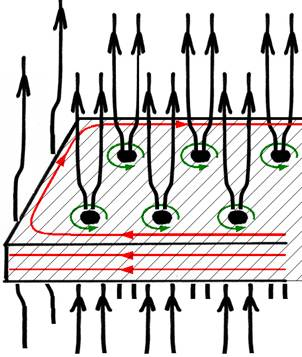
\includegraphics[width=0.25\textwidth]{estado_mixto} 
				\caption{Representaci\'{o}n del estado mixto. Se aplica un campo magn\'{e}tico
				(en negro). Las corrientes superconductoras (en rojo) se desarrollan en
				la superficie para hacer una pantalla contra este campo; esas son las
				corrientes responsables del efecto Meissner. Se desarrollan otras
				corrientes superconductoras (en verde) que crean v\'{o}rtices (como
				``t\'{u}neles'' no superconductores). Estos v\'{o}rtices permiten que una cantidad
				de flujo magn\'{e}tico pase a trav\'{e}s de ellos y, por lo tanto, permita que
				parte del campo magn\'{e}tico aplicado pase a trav\'{e}s de la muestra
				superconductora.
				} 
				\label{fig:estado_mixto}
\end{figure}

Se produce un efecto similar
sobre la inclusi\'{o}n de material no superconductor, que proporciona una regi\'{o}n de
$T_c$ suprimida que puede estar muy localizada o bastante extendida, dependiendo de
la naturaleza de la inclusi\'{o}n; sin embargo, dicha inclusi\'{o}n tambi\'{e}n constituye
un defecto material que tendr\'{a} un efecto de dispersi\'{o}n en los portadores de
carga, actuando para variar el camino libre medio electr\'{o}nico. %, $l$.
%(pin $\delta l$, anteriormente denominado $\delta \kappa$ pinning [2]). 
En todos los casos, el resultado es el mismo: la creaci\'{o}n de un sitio de
menor energ\'{i}a (preferido) para la ocupaci\'{o}n del v\'{o}rtice.

Para un efecto m\'{a}ximo, las variaciones espaciales deben ocurrir en la escala
de longitud de $\xi$ o $ \lambda$. 
Las modificaciones a peque\~{n}a escala, como las
sustituciones at\'{o}micas, pueden crear inhomogeneidades a gran escala a
trav\'{e}s de alteraciones de la estructura electr\'{o}nica o la creaci\'{o}n de
campos de tensi\'{o}n. Es el alcance de la falta de
homogeneidad, no el alcance de la modificaci\'{o}n, lo que importa.  

Se puede
hacer una distinci\'{o}n \'{u}til entre las fuerzas de anclaje que operan sobre
la escala de longitud de $\xi$
%, denominada anclaje de n\'{u}cleo (v\'{o}rtice),
y las que operan sobre una escala de longitud de $\lambda$.
%, denominada anclaje magn\'{e}tico
A la primera categor\'{i}a pertenecen la mayor\'{i}a de los
centros de fijaci\'{o}n artificial exitosamente empleados hasta la fecha,
as\'{i} como todos los defectos comunes de crecimiento, mientras que la
\'{u}ltima categor\'{i}a comprende fuentes naturales como superficies extendidas
y poros donde el flujo entra o sale por completo del superconductor, as\'{i}
como la fijaci\'{o}n debida a las interacciones v\'{o}rtice-v\'{o}rtice.
Si bien las interacciones v\'{o}rtice-v\'{o}rtice act\'{u}an para fijar v\'{o}rtices, es
importante tener en cuenta que esto solo puede ocurrir si al menos algunos de
los v\'{o}rtices est\'{a}n anclados por otra fuente; de lo contrario, todo el
conjunto simplemente se deslizar\'{a} a trav\'{e}s del material.

\begin{figure}[!ht]
				\centering 
				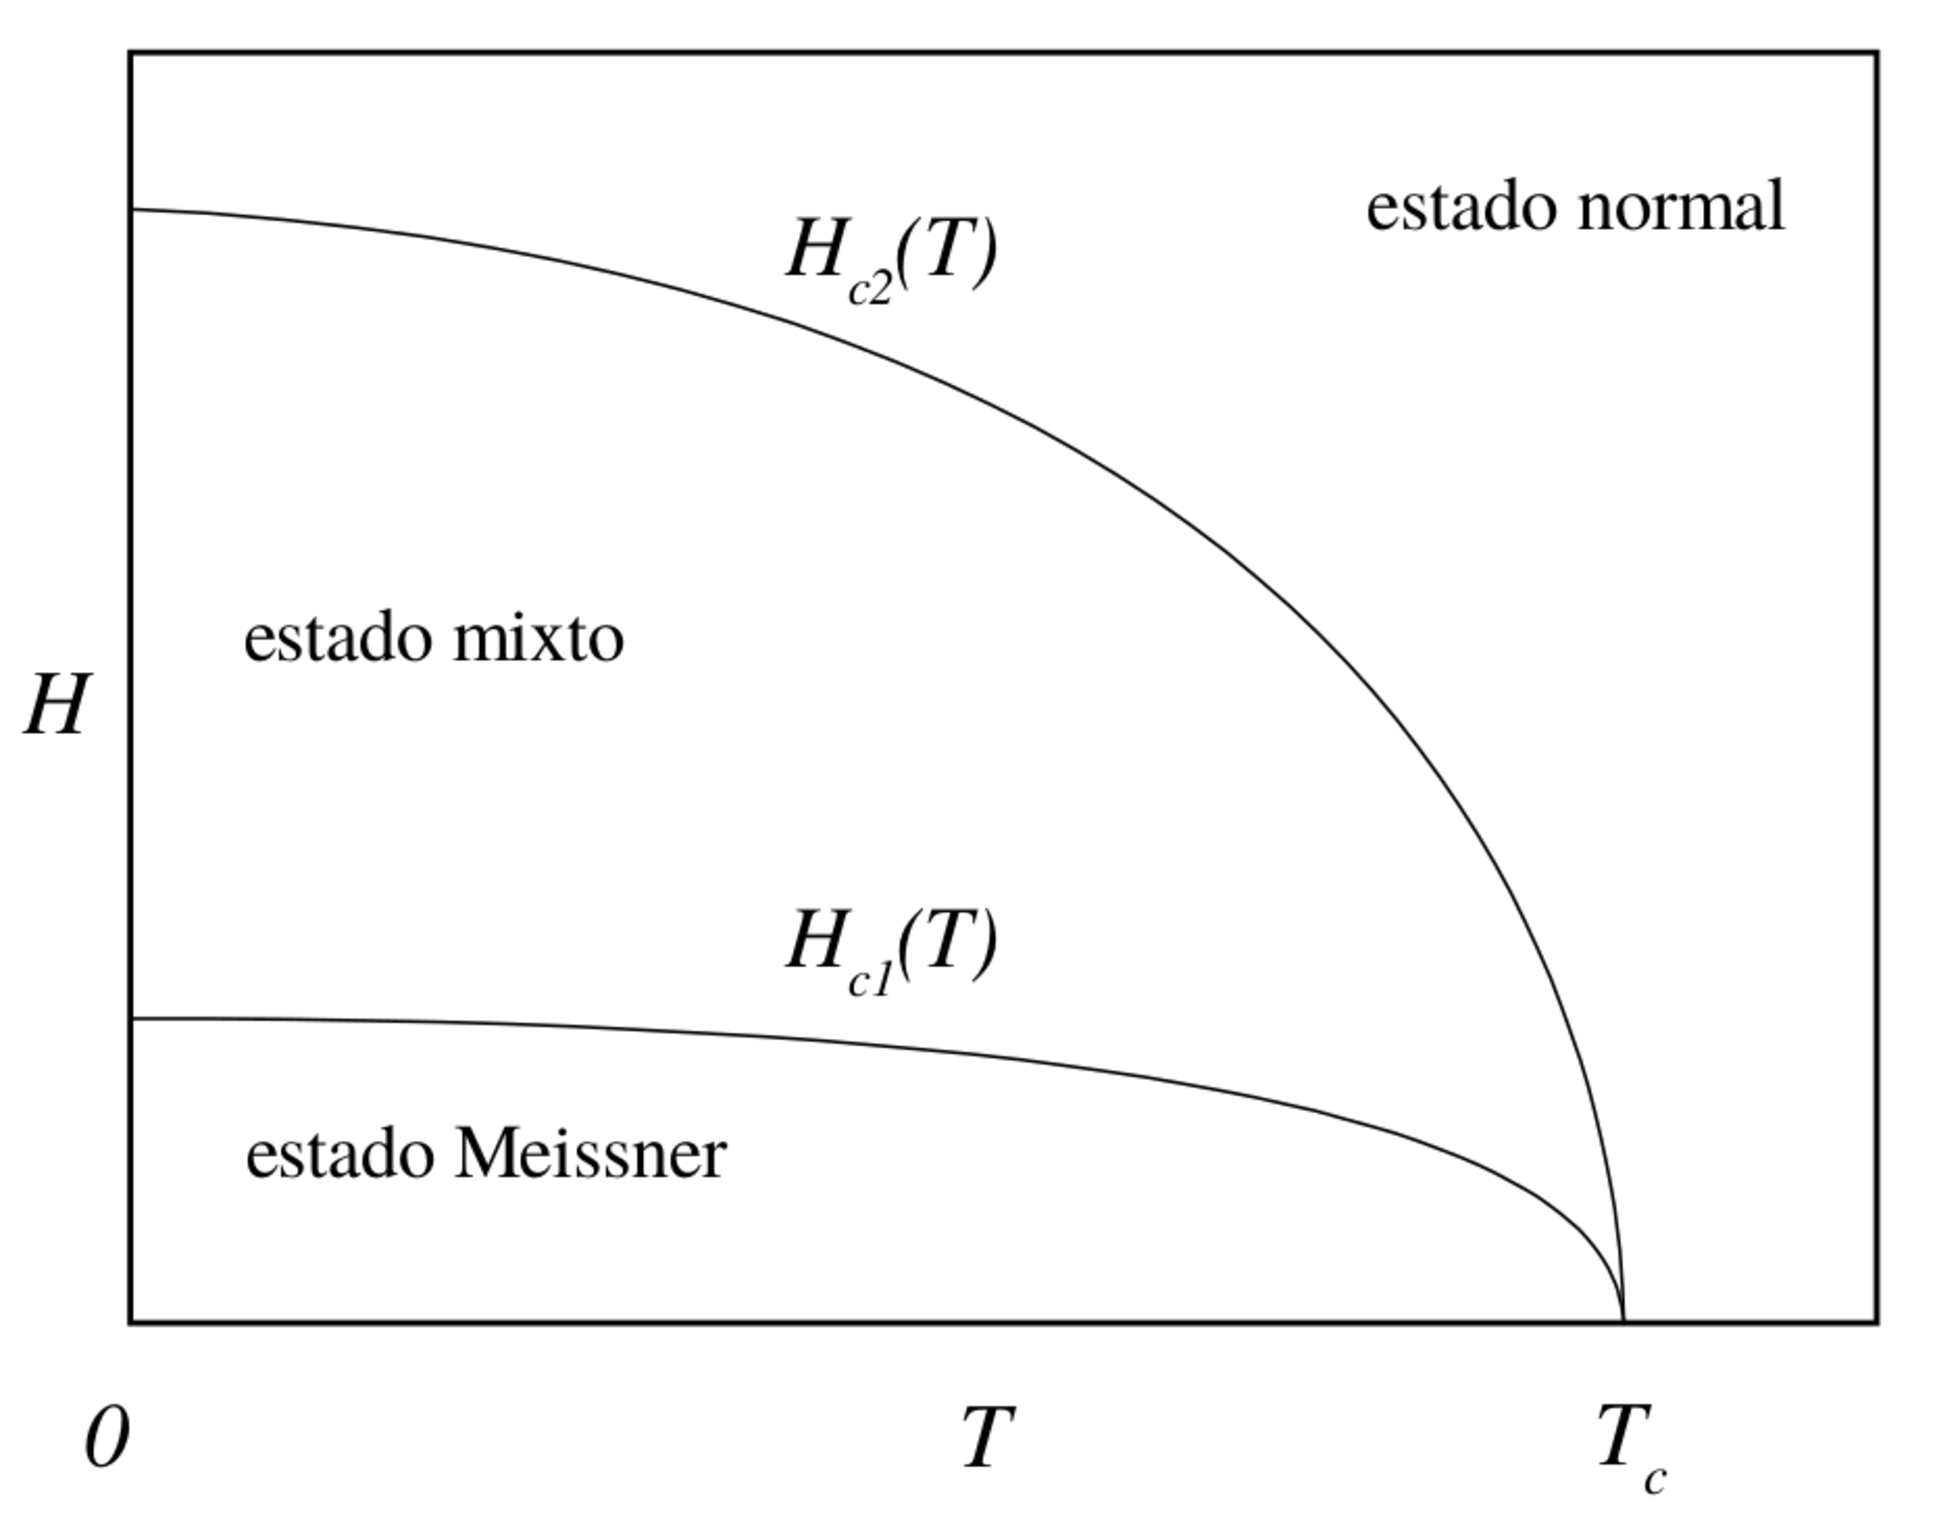
\includegraphics[width=0.37\textwidth]{diagrama_fase_HT} 
				\caption{Diagrama de fases de campo medio que comprende una fase met\'{a}lica
				normal en campos y temperaturas altas, separados por la l\'{i}nea de campo
				cr\'{i}tico superior $H_{c_2}(T)$ de la fase mixta, que a su vez
				est\'{a} separada por el campo cr\'{i}tico inferior l\'{i}nea $H_{c_1}(T)$ desde la fase
				Meissner-Ochsenfeld a bajas temperaturas y campos.
				} 
				\label{fig:diagrama_fase_ht}
\end{figure}

%Por definici\'{o}n, todas estas inhomogeneidades espaciales constituyen defectos en
%la red cristalina del superconductor, por lo que la fijaci\'{o}n de flujo est\'{a} unida
%inextricablemente a la estructura del defecto del material.
%Como consecuencia, 
La ingenier\'{i}a de defectos de materiales tecnol\'{o}gicamente relevantes
forma un extenso campo de trabajo. Es com\'{u}n catalogar los tipos disponibles
de defectos de anclaje y una clasificaci\'{o}n \'{u}til es enumerarlos en
t\'{e}rminos de su dimensionalidad, como se observa en la
\figurename~\ref{fig:tipos_defectos}. Los defectos unidimensionales (en
l\'{i}nea o en columnas) incluyen dislocaciones y defectos artificiales, como
las huellas de da\~{n}os resultantes de la irradiaci\'{o}n de iones pesados,
neutrones o protones. Son una clase particularmente interesante desde el punto
de vista de la fijaci\'{o}n de flujo debido a su congruencia con la forma de la
l\'{i}nea de flujo en s\'{i}. La correlaci\'{o}n entre los defectos y las
l\'{i}neas de flujo puede llevar a un anclaje extremadamente fuerte, y la
l\'{i}nea de flujo se fija a lo largo de toda su longitud.  La microscop\'{i}a
electr\'{o}nica de alta resoluci\'{o}n confirma la formaci\'{o}n de pistas
lineales de material altamente defectuoso alineado con la direcci\'{o}n del haz.
La estructura del defecto resultante se puede modelar como una matriz aleatoria
de cilindros normales paralelos de di\'{a}metro $50 - 70\,\textup{\r{A}}$
incrustados en una matriz de material superconductor. La densidad de estas
columnas se mide convenientemente en t\'{e}rminos del campo de matching, $
B_\Phi $, que produce una densidad equivalente de l\'{i}neas de v\'{o}rtice en
el superconductor. Las dosis de irradiaci\'{o}n t\'{i}picas utilizadas en los
experimentos producen valores para $ B_ \Phi $ entre 1 y 5 T.

%Como ejemplo, las dislocaciones tipo tornillos
%que surgen naturalmente durante el crecimiento de las pel\'{i}culas delgadas de
%\'{o}xido de itrio, bario y cobre (YBCO), formando parte del modo de crecimiento
%del material y contribuyen en gran medida a su alto $J_c$ incluso antes de la
%modificaci\'{o}n microestructural. 
%Se aplica un fuerte enfoque a la
%ingenier\'{i}a de centros de fijaci\'{o}n artificial de este tipo en un intento
%de suavizar la anisotrop\'{i}a de $J_c$ que se produce naturalmente en los
%materiales HTS. 

Dado que las t\'{e}cnicas de irradiaci\'{o}n de alta energ\'{i}a
no son pr\'{a}cticas para la producci\'{o}n industrial, el \'{e}nfasis est\'{a}
en los procesos de autoensamblaje de las inclusiones de la segunda fase, aunque
se han empleado m\'{e}todos de implantaci\'{o}n de iones de baja energ\'{i}a con
cierto \'{e}xito en la introducci\'{o}n de grupos de \'{a}tomos que act\'{u}an
como centros de fijaci\'{o}n volum\'{e}tricos.

La efectividad de los defectos columnares para el anclaje de los v\'{o}rtices en
superconductores de alta temperatura cr\'{i}tica es conocida desde hace m\'{a}s
de veinte a\~{n}os, cuando se observ\'{o} un fuerte aumento de la corriente
cr\'{i}tica y de la extensi\'{o}n de la zona de irreversibilidad en muestras
irradiadas con iones de Pb \cite{Marwick1991, Konczykowski1991}.  La densidad en
el n\'{u}mero de defectos columnares se mide en t\'{e}rminos del campo de
matching, que corresponde al valor de la inducci\'{o}n magn\'{e}tica tal que el
n\'{u}mero de v\'{o}rtices es igual al n\'{u}mero de defectos 

\begin{equation}
				\label{eq:matching_field}
				B_\Phi = n_d \Phi_0\,,
\end{equation}

\noindent donde $n_d$ es la densidad de columnares por unidad de \'{a}rea en el
plano ab y $\Phi_0$ es el cuanto de flujo magn\'{e}tico definido en
\ref{eq:cuanto_flujo_magnetico}.

\begin{figure}[!ht]
				\centering 
				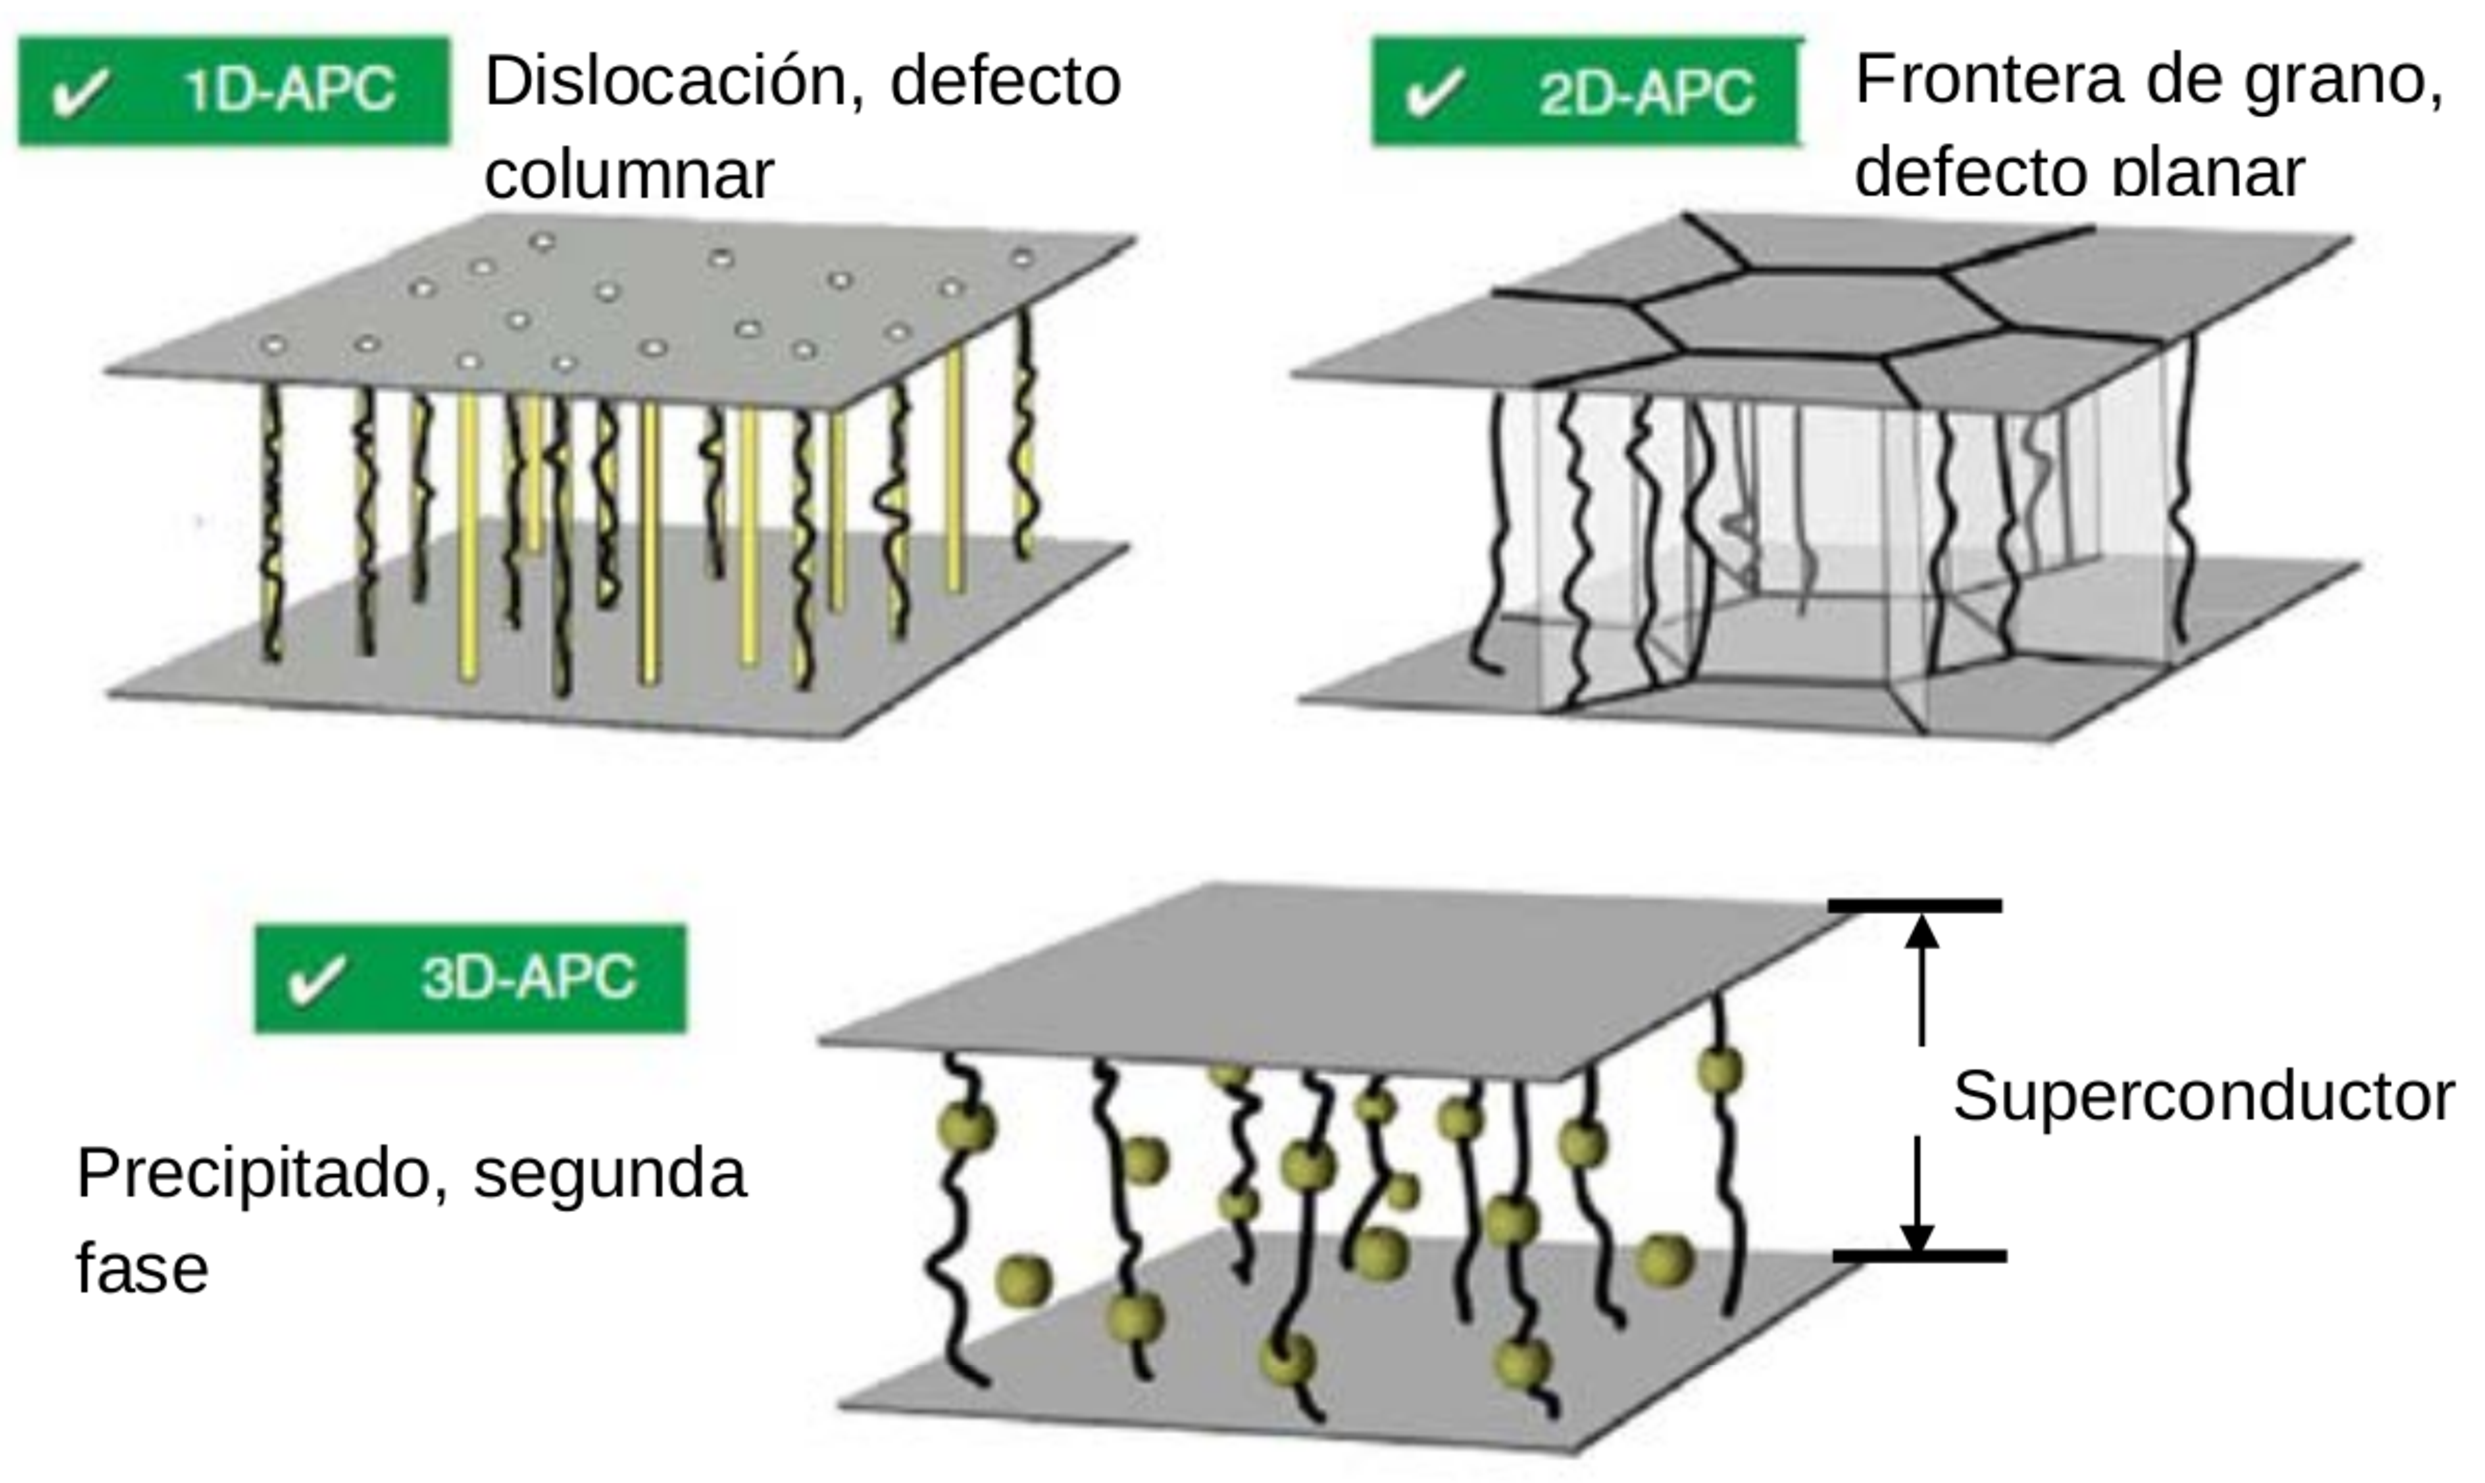
\includegraphics[width=0.47\textwidth]{tipos_defectos_1D_2D_3D} 
				\caption{Ilustraci\'{o}n esquem\'{a}tica del anclaje de l\'{i}neas de flujo por
				defectos cristalinos de dimensionalidad variable.
				} 
				\label{fig:tipos_defectos}
\end{figure}

%The following sections describe the design criteria used in order to contruct
%the polyphase filter bank channelizer. Section~\ref{sec:DFB} gives an overview of the
%digital filter banks. In Section~\ref{sec:polyphase_structure_of_DFT_PFB}
%details are given for the structure and working principles of the DFT polyphase
%filter bank. Section~\ref{sec:pf_design} summarizes the design criteria for the
%implementation of the channelizer's prototype filter. The results for simulations
%and the implementation of the channelizer in the RedPitaya board are presented
%in Section~\ref{sec:simulations_and_testing}.
%Finally, conclusions are provided in Section~\ref{sec:conclusions}.

%\begin{equation}
%				\label{eq:parametro_red}
%				a_0 = 1.075 \sqrt{\frac{\Phi_0}{B}}
%\end{equation}

%Tomado de la tesis de Albornoz
%Los v\'{o}rtices interact\'{u}an fuertemente con
%los defectos de la red cristalina del sustrato en el que se encuentran. Una
%forma de estudiar estas interacciones consiste en generar artificialmente
%defectos en el material. Existen diversas formas de generar estos defectos, y
%cada una los produce con distintas caracter\'{i}sticas: pueden ser puntuales,
%correlacionados, y con distintas distribuciones espaciales.  
%%En nuestro trabajo,
%%estudiamos muestras de Bi-2212 que est\'{a}n irradiadas con iones de Xe
%%acelerados a una energ\'{i}a de 1 GeV. 
%Estos iones atraviesan la muestra en la
%direcci\'{o}n del eje c de la estructura cristalina, generando defectos
%columnares que est\'{a}n orientados en esa direcci\'{o}n y distribuidos de forma
%aleatoria. Los defectos columnares son ''columnas`` de radio $\sim$ 3 nm en las
%que la red cristalina del material est\'{a} amorfizada.  Los defectos columnares
%en la direcci\'{o}n del eje c son centros de anclaje muy efectivos para los
%v\'{o}rtices cuando el campo magn\'{e}tico est\'{a} aplicado en esa
%direcci\'{o}n. Esto ocurre fundamentalmente por el hecho de que son defectos
%lineales, y las l\'{i}neas de flujo son capaces de ubicarse en su totalidad a lo
%largo de ellos, encontrando as\'{i} una condici\'{o}n muy favorable
%energ\'{e}ticamente. Esto los diferencia de los defectos puntuales que existen
%naturalmente en cualquier estructura cristalina. 
%La efectividad de los defectos
%columnares para el anclaje de los v\'{o}rtices en superconductores de alta
%temperatura cr\'{i}tica es conocida desde hace m\'{a}s de veinte a\~{n}os, cuando se
%observ\'{o} un fuerte aumento de la corriente cr\'{i}tica y de la extensi\'{o}n de
%la zona de irreversibilidad en muestras irradiadas con iones de Pb
%\cite{Marwick1991, Konczykowski1991}.  La densidad en el n\'{u}mero de defectos
%columnares se mide en t\'{e}rminos del campo de conmensurabilidad, o campo de
%matching, $B_\Phi$ , que corresponde al valor de la inducci\'{o}n magn\'{e}tica
%tal que el n\'{u}mero de v\'{o}rtices es igual al n\'{u}mero de defectos. Es
%decir,
%
%\begin{equation}
%				\label{eq:matching_field}
%				B_\Phi = n_d \Phi_0
%\end{equation}
%
%donde $n_d$ es la densidad de columnares por unidad de \'{a}rea en el plano ab y
%$\Phi_0$ es el
%cuanto de flujo magn\'{e}tico definido en \ref{eq:quantum_flux}.

\subsection{Modificaci\'{o}n del diagrama de fases}

El efecto de la introducci\'{o}n de altas densidades de defectos columnares
($B_\Phi \sim kG$) en superconductores de alta temperatura cr\'{i}tica ha sido muy
estudiado debido fundamentalmente al inter\'{e}s pr\'{a}ctico de aumentar la
corriente cr\'{i}tica de estos materiales \cite{Marwick1991, Konczykowski1991}. En
estos casos se observ\'{o} que el paso del l\'{i}quido al s\'{o}lido de v\'{o}rtices
se da a trav\'{e}s de una transici\'{o}n continua, similar a la de depinning.
Como los defectos columnares est\'{a}n distribuidos de manera aleatoria, si la
energ\'{i}a de anclaje es m\'{a}s relevante que la energ\'{i}a el\'{a}stica la fase
s\'{o}lida de v\'{o}rtices es una fase amorfa. 
%En este contexto, la fase
%ordenada de la que hablamos en la secci\'{o}n 1.3, limitada por una
%transici\'{o}n de primer orden, no es estable.

%tomado de la pagina https://www.fisicanet.com.ar/tecnicos/tecnologia/te11_superconductividad.php
%Las maclas pertenecen a una clase de defectos denominados correlacionados que
%han jugado un papel muy importante en la superconductividad de alta temperatura.

%tomado del review de Blatter puede ser la introduccion de todo porque viene de
%la seccion defectos columnares
%El anclaje en un superconductor de tipo II se puede optimizar introduciendo
%defectos que atrapan las l\'{i}neas de v\'{o}rtice individuales a lo largo de sus
%dimensiones lineales y, al mismo tiempo, destruyen una fracci\'{o}n de volumen
%m\'{i}nimo del material superconductor en s\'{i}. Claramente, una estructura defectuosa
%que alcanza este objetivo se puede obtener introduciendo defectos columnares en
%el material con cilindros de material no superconductor de di\'{a}metro $\sim
%\xi$, el tama\~{n}o del n\'{u}cleo del v\'{o}rtice. Las propiedades de anclaje
%resultantes
%ser\'{a}n altamente anisotr\'{o}picas, obteni\'{e}ndose un anclaje \'{o}ptimo para una
%configuraci\'{o}n en la que el campo magn\'{e}tico est\'{a} alineado con la estructura
%lineal de defectos. Para esta situaci\'{o}n, cada v\'{o}rtice atrapado gana una energ\'{i}a
%$U_r = \alpha H_c^2 \xi^2 L $, donde L es el tama\~{n}o del sistema a lo
%largo de la direcci\'{o}n del campo magn\'{e}tico y a es un factor de geometr\'{i}a. Para
%campos tan d\'{e}biles que los defectos superan a los v\'{o}rtices y la interacci\'{o}n
%entre los v\'{o}rtices es insignificante en comparaci\'{o}n con $U_r$, podemos esperar
%obtener una densidad de corriente cr\'{i}tica $j_c \lesssim \alpha j_o$, $\alpha
%\sim 0.1 - 1$, de el orden de la densidad de corriente de depairing $j_o$.  En segundo
%lugar, dado que el ablandamiento t\'{e}rmico del potencial de pineado lineal es
%mucho m\'{a}s gradual que para los pines en forma de punto, tambi\'{e}n se puede esperar
%una disminuci\'{o}n menor de la densidad de corriente cr\'{i}tica con el aumento de la
%temperatura. Ambos efectos han sido observados por Civale et al. (1991) y por
%Konczykowski, Rullier-Albenque et al. (1991) en muestras de YBCO irradiadas con
%iones Sn y Pb de alta energ\'{i}a ($\sim GeV$). Los iones pesados
%r\'{a}pidos producen pistas lineales de material da\~{n}ado debido a su gran
%tasa de p\'{e}rdida de energ\'{i}a de ionizaci\'{o}n grande, que excede algunos
%$keV/\textup{\r{A}}$. La
%microscop\'{i}a electr\'{o}nica de alta resoluci\'{o}n confirma la formaci\'{o}n de pistas
%lineales de material altamente defectuoso alineado con la direcci\'{o}n del haz. La
%estructura del defecto resultante se puede modelar como una matriz aleatoria de
%cilindros normales paralelos de di\'{a}metro $50 - 70\,\textup{\r{A}}$ incrustados en una matriz de
%material superconductor. La densidad de estas columnas se mide convenientemente
%en t\'{e}rminos del campo $ B_\Phi $ (el "campo coincidente") que produce una
%densidad equivalente de l\'{i}neas de v\'{o}rtice en el superconductor. Las dosis de
%irradiaci\'{o}n t\'{i}picas utilizadas en los experimentos producen valores para $ B_ \Phi $ entre 1 y 5 T.

%tomado del review de Blatter
%Finalmente, analicemos brevemente las principales consecuencias de la fijaci\'{o}n
%fuerte, cuyos ejemplos se dan en los l\'{i}mites gemelos en YBCO, por dislocaciones
%de tornillo producidas en pel\'{i}culas delgadas durante el crecimiento o por
%defectos columnares introducidos artificialmente. El tipo de fijaci\'{o}n fuerte que
%es tecnol\'{o}gicamente m\'{a}s relevante (y que es f\'{i}sicamente muy interesante) se
%obtiene irradiando el material con iones de alta energ\'{i}a. Las pistas lineales
%del material da\~{n}ado introducen entonces un trastorno fuertemente correlacionado
%en el sistema de v\'{o}rtice (alineado). En campos magn\'{e}ticos bajos, de manera que
%$a_o \gg d_r$, donde $d_r$ denota la distancia media entre las pistas, cada
%v\'{o}rtice se fija individualmente por un defecto columnar. Como la energ\'{i}a de
%anclaje ahora crece linealmente con la distancia, el anclaje se vuelve fuerte y
%la densidad de corriente cr\'{i}tica $j_c$ toma valores cercanos a su l\'{i}mite
%superior, $j_c \leq j_o$. Mientras que a bajas temperaturas cada l\'{i}nea de v\'{o}rtice
%est\'{a} unida a su defecto de l\'{i}nea, los v\'{o}rtices tienden a deslocalizarse al
%aumentar la temperatura. A medida que el promedio de desplazamiento t\'{e}rmico $
%\langle u^2 \rangle^{1/2}_{th}$ se vuelve igual a la distancia $ d_r $ entre las
%pistas, el v\'{o}rtice se fija colectivamente por un conjunto de defectos de l\'{i}nea.
%Luego se reduce la fijaci\'{o}n, ya que solo las fluctuaciones en la densidad de las
%pistas conducen a la fijaci\'{o}n de la l\'{i}nea de v\'{o}rtice. Es interesante comparar la
%competencia entre el trastorno t\'{e}rmico y el inactivado para los dos casos en los
%que una sola l\'{i}nea de v\'{o}rtice est\'{a} fijada colectivamente por un trastorno no
%correlacionado (puntual) y por un trastorno correlacionado (defectos de l\'{i}nea):
%una l\'{i}nea de v\'{o}rtice sujeta a un trastorno puntual no correlacionado y
%fluctuaciones t\'{e}rmicas se fija en 3D, y por lo tanto, la densidad cr\'{i}tica de
%corriente solo marginalmente se desvanece exponencialmente con el aumento de la
%temperatura. Por otro lado, el trastorno correlacionado compite m\'{a}s
%eficientemente con las fluctuaciones t\'{e}rmicas, resultando en un decaimiento
%algebraico m\'{a}s d\'{e}bil de la densidad de corriente cr\'{i}tica al aumentar la
%temperatura.
%Otra diferencia interesante entre el trastorno no correlacionado y el trastorno
%correlacionado es que, en el primer caso, la mec\'{a}nica estad\'{i}stica del v\'{o}rtice se
%caracteriza por el desv\'{i}o de l\'{i}neas, mientras que en el \'{u}ltimo caso el rasgo
%caracter\'{i}stico es la localizaci\'{o}n.
%En lo que sigue, se har\'{a} un recorrido por los diferentes trabajos realizados 

\section{Dispersi\'{o}n angular en la direcci\'{o}n de los defectos
columnares}\label{sec:splay}

El estudio de la dependencia angular en la fijaci\'{o}n de v\'{o}rtices en
superconductores de alta temperatura (HTSC) con defectos columnares ha revelado
una variedad m\'{a}s rica de fen\'{o}menos y reg\'{i}menes de fijaci\'{o}n de lo
que originalmente se esperaba.
%tomado del paper de Hwa
En el trabajo presentado por T. Hwa \textit{et. al.} en~\cite{Hwa1994} se
propone la dispersi\'{o}n angular (splay) controlada de defectos columnares
artificiales en cupratos superconductores como una estrategia para mejorar las
propiedades de transporte en comparaci\'{o}n con defectos columnares paralelos.
Dicha dispersi\'{o}n est\'{a} presente intr\'{i}nsecamente en cualquier proceso
de irradiaci\'{o}n, y puede amplificarse experimentalmente oscilando la muestra
durante la irradiaci\'{o}n.  Nelson y Vinokur~\cite{Nelson1993} consideraron la
teor\'{i}a de la fijaci\'{o}n de l\'{i}neas de flujo mediante columnas paralelas
rectas, quienes demostraron que la f\'{i}sica a baja temperatura es id\'{e}ntica
a la del vidrio Bose~\cite{Fisher1989}, con l\'{i}neas de flujo fuertemente
localizadas en los defectos columnares, resultando en cero resistividad en DC.

En el art\'{i}culo de T. Hwa \textit{et. al.}~\cite{Hwa1994}, los autores se
apoyan en la predicci\'{o}n te\'{o}rica de una nueva fase de ``vidrio
extendido'', caracterizado por una fluencia de flujo reducido, un estado
fundamental enredado y una respuesta lenta a un campo transversal aplicado.  
%El vidrio extendido tiene algunas similitudes con el vidrio Bose convencional:
%la f\'{i}sica est\'{a} dominada por la localizaci\'{o}n a lo largo de defectos
%columnares.  ; as\'{i} se pueden construir excitaciones de baja energ\'{i}a
%mediante adaptaciones de las ideas de salto de alcance variable. 
Adem\'{a}s, el aumento dram\'{a}tico observado en la magnitud de $H_{irr}(T)$
deber\'{i}a reducirse apenas ligeramente con una peque\~{n}a dispersi\'{o}n.
Sin embargo, el vidrio extendido difiere del vidrio Bose en al menos dos
aspectos importantes, los cuales deber\'{i}an mejorar las propiedades de
transporte. Primero, las desorientaciones aleatorias de las columnas inhiben
fuertemente las excitaciones a gran escala y de baja energ\'{i}a. En segundo
lugar, las l\'{i}neas de flujo en el estado fundamental del vidrio extendido
est\'{a}n enredadas, en un claro contraste con el estado fundamental del vidrio
Bose, el cual es no-enredado, ver \figurename~\ref{fig:splay_de_vortices}.

%Encontramos que los defectos columnares dispersos conducen a una
%nueva fase de vidrio, con propiedades de transporte mejoradas a medida que $J
%\to 0$, y un entrelazamiento de l\'{i}neas de v\'{o}rtice en forma de
%pol\'{i}mero. Si la dispersi\'{o}n es peque\~{n}a, esta mejora en el transporte y el
%entrelazado estar\'{a}n acompa\~{n}ados por una
%modesta reducci\'{o}n en la temperatura de transici\'{o}n del vidrio Bose.
En resumen, puede ser posible producir los efectos de fijaci\'{o}n de flujo
m\'{a}s fuertes hasta ahora conocidos simplemente dispersando angularmente los
defectos columnares que responden din\'{a}micamente a una peque\~{n}a
inclinaci\'{o}n.

\begin{figure}[!ht]
				\centering 
				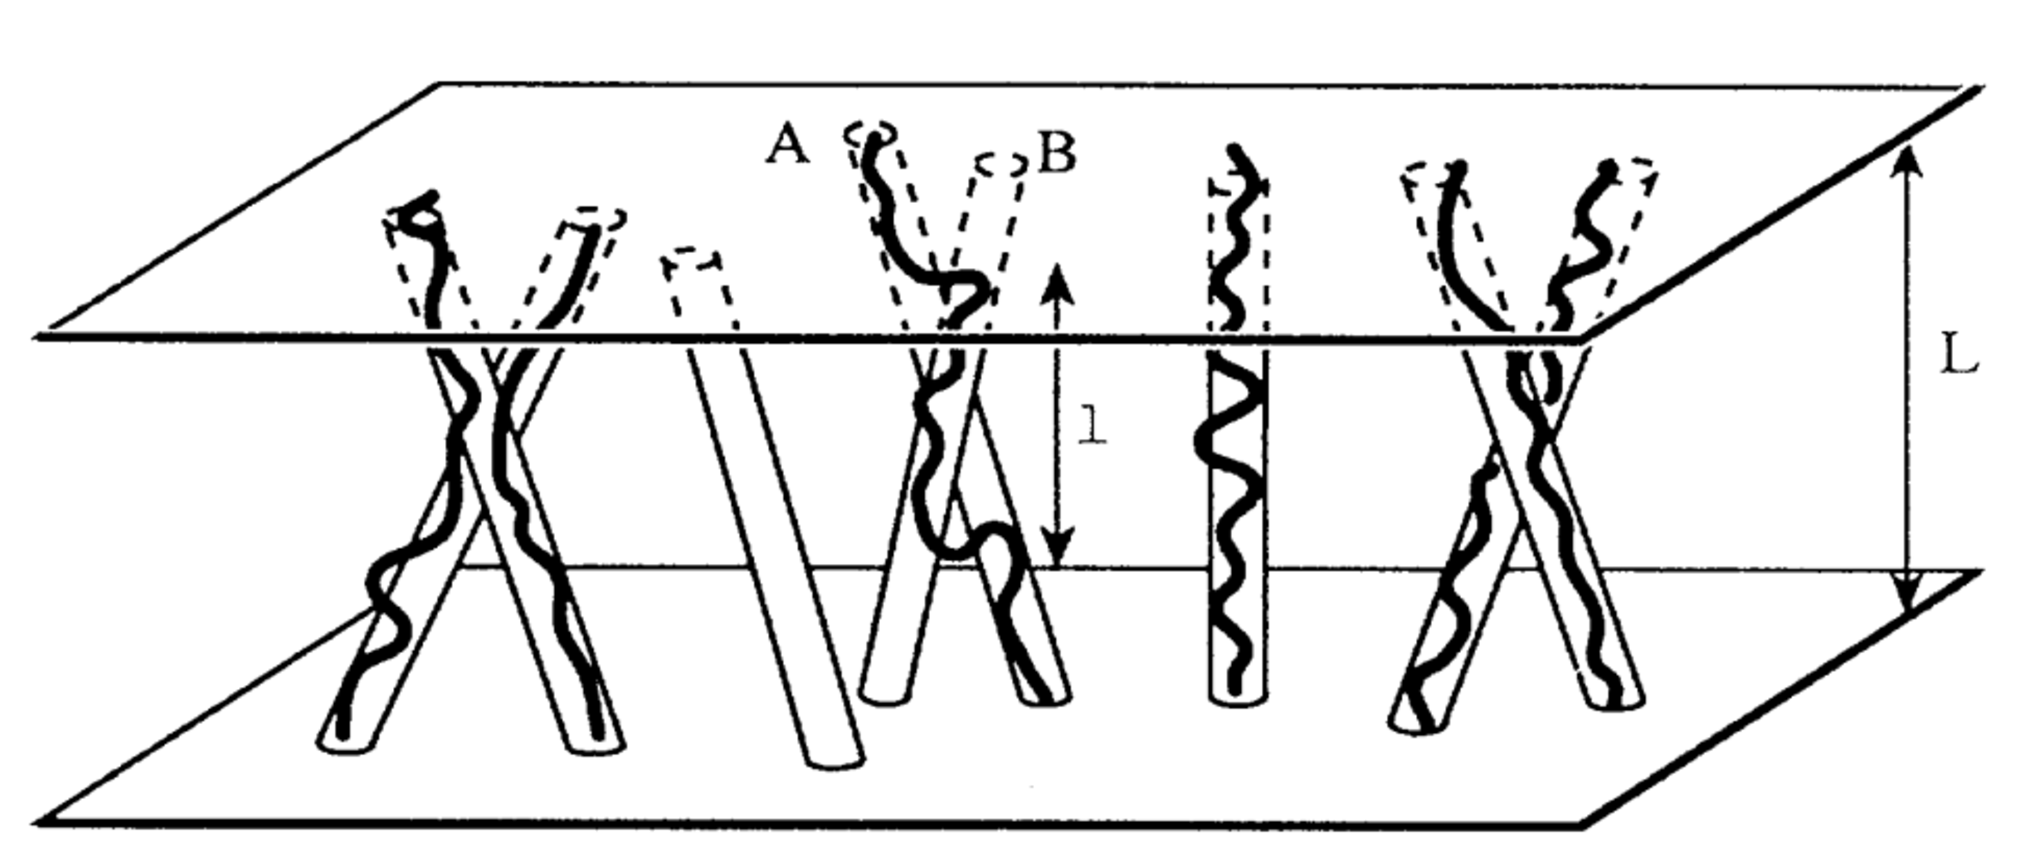
\includegraphics[width=0.42\textwidth]{splay_de_vortices} 
				\caption{Ilustraci\'{o}n de las configuraciones del estado fundamental. Las
				l\'{i}neas de flujo se localizan en pines inclinados a la derecha (un
				proceso ``directo''), con un proceso de ``intercambio'' a la izquierda.
				Tambi\'{e}n se muestra una excitaci\'{o}n de doble torsi\'{o}n entre los
				pines A y B~\cite{Hwa1994}.
				} 
				\label{fig:splay_de_vortices}
\end{figure}

\begin{figure}[!ht]
				\centering 
				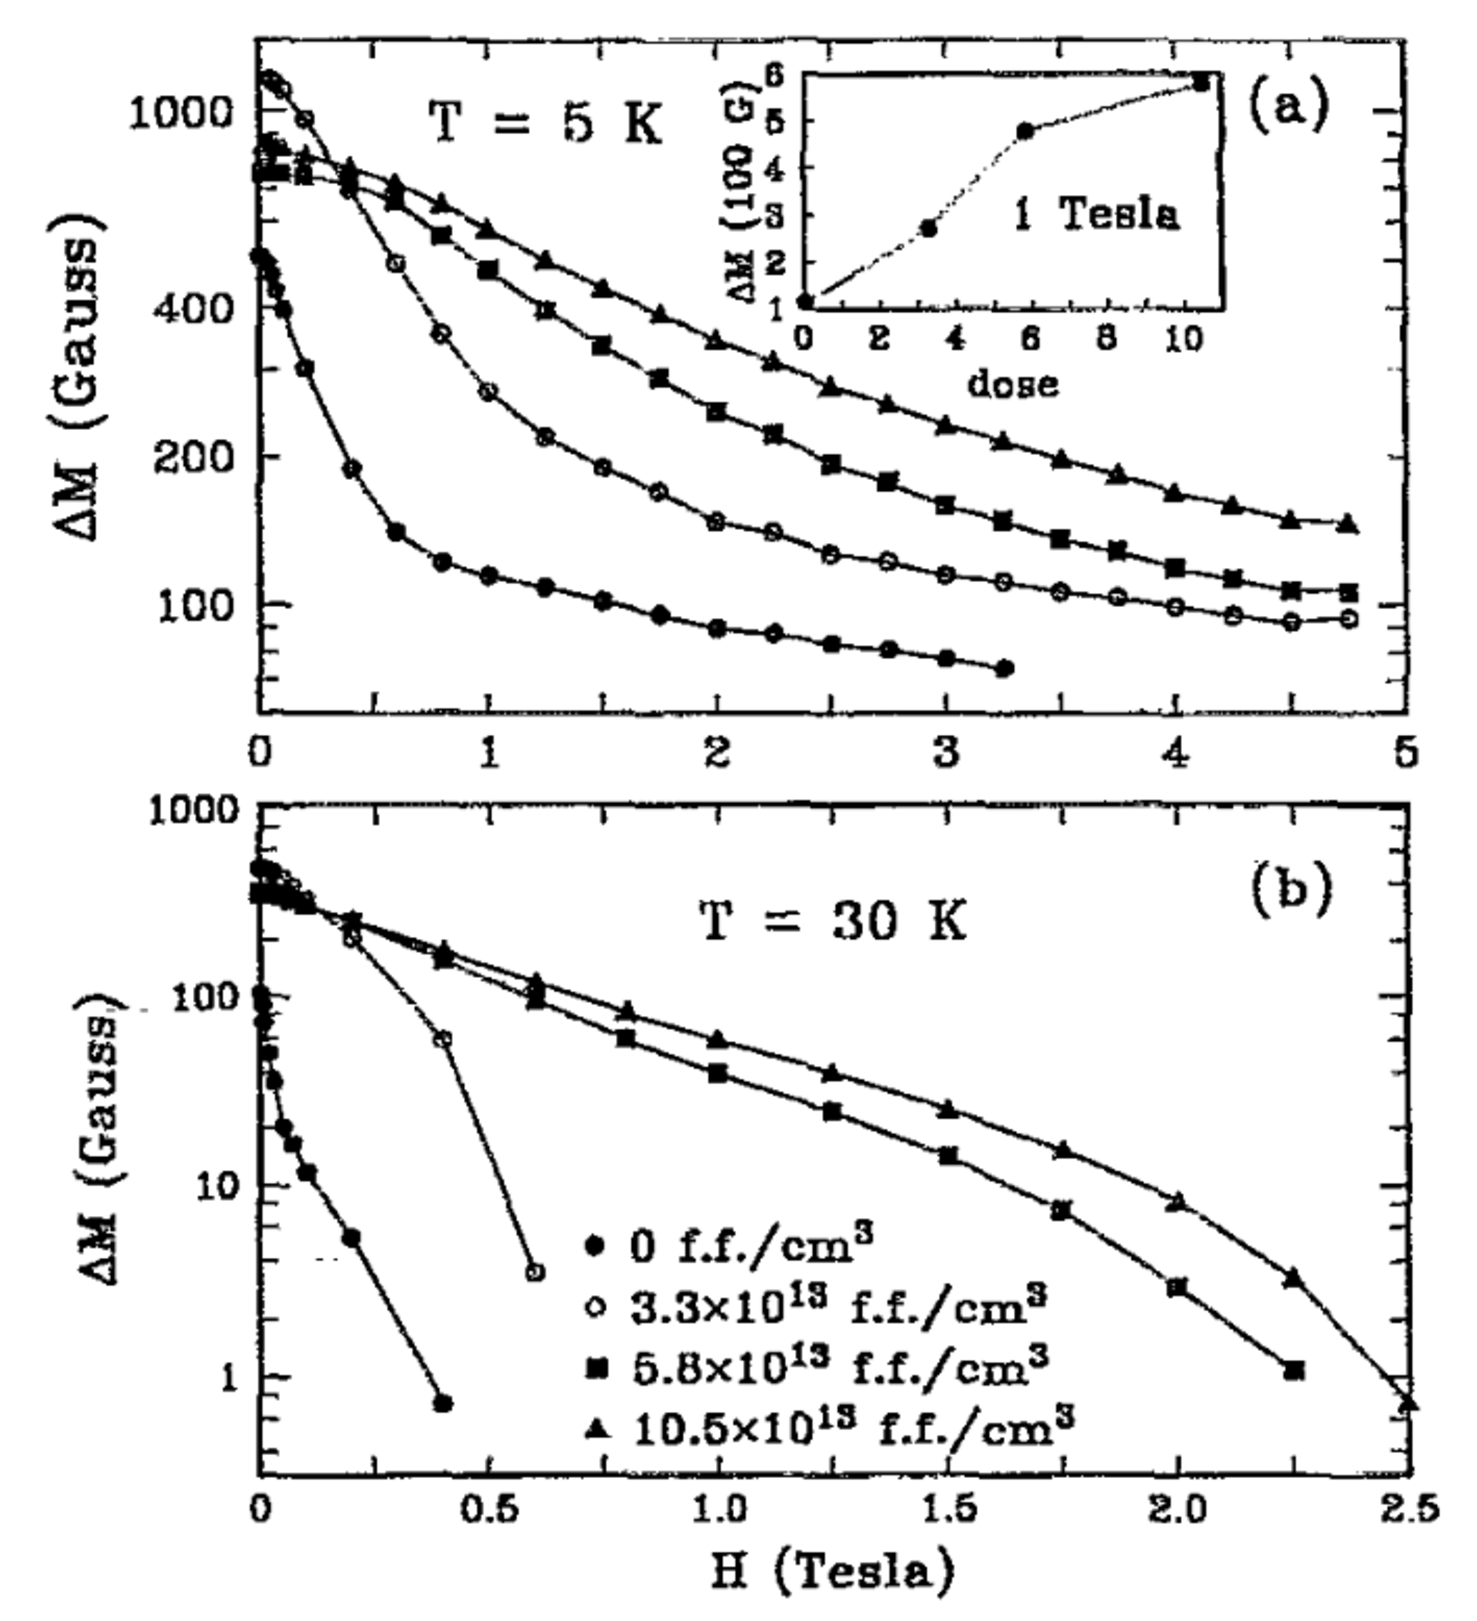
\includegraphics[width=0.42\textwidth]{splay2}
				\caption{
								Ancho del loop de hist\'{e}resis magn\'{e}tica $\Delta M$ vs campo aplicado
								para las cintas de Bi-2212/Ag orientadas en el eje c antes y despu\'{e}s
								de la irradiaci\'{o}n con protones de $0.8\,\text{GeV}$ a $T =
								5\,\text{K}$ (a) y a $T = 30\,\text{K}$ (b). Las densidades de
								fisi\'{o}n de 3.3, 5.8 y $10.5\times10^{13}\,\text{f.f./cm}^3$
								corresponden a densidades de \'{a}rea de 2.0, 3.5 y
								$6.5\times10^{10}\,\text{f.f./cm}^2$, respectivamente. El
								recuadro muestra una gr\'{a}fica lineal de $\Delta M$ vs dosis
								(en unidades de $10^{13}/\text{cm}^3$) en el campo aplicado de
								$\text{H} =
								1\,\text{T}$~\cite{Krusin-Elbaum1994}.
				} 
				\label{fig:splay2}
\end{figure}

\begin{figure}[!ht]
				\centering 
				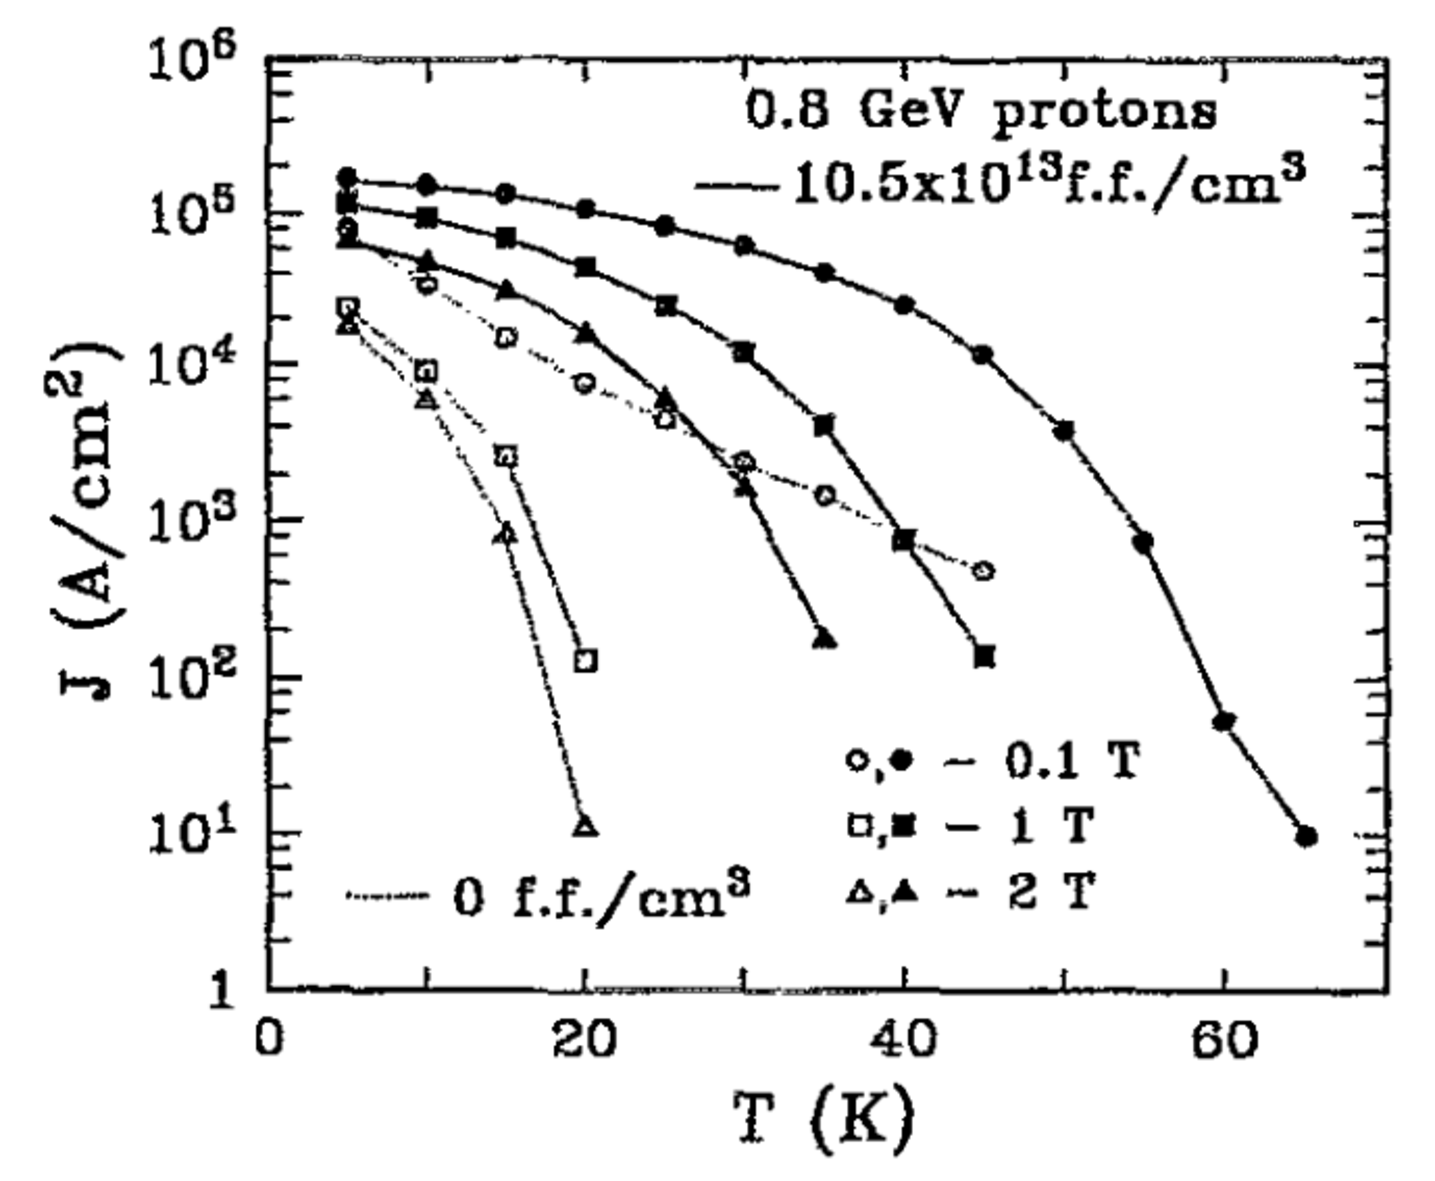
\includegraphics[width=0.42\textwidth]{splay1}
				\caption{
								Densidad de corriente persistente J vs temperatura para una muestra de cinta de  
				Bi-2212 tal como se sintetiz\'{o} y despu\'{e}s del procesamiento con $6.5
				\times 10^{10}\, \text{f.f./cm}^2$. Se
				aplicaron tres valores de campo magn\'{e}tico normales a la cinta. Despu\'{e}s de la
				irradiaci\'{o}n, J se hace grande por encima de la l\'{i}nea de irreversibilidad de la
				cinta sin irradiar~\cite{Krusin-Elbaum1994}.
				} 
				\label{fig:splay1}
\end{figure}

Los trabajos presentados en \cite{Civale1994, Krusin-Elbaum1994,
Krusin-Elbaum1996, Kwok1998} confirmaron experimentalmente esta teor\'{i}a.
En el trabajo de Krusin-Elbaum \textit{et. al.}~\cite{Krusin-Elbaum1994} se
irradiaron cintas compuestas del superconductor $Bi_2 Sr_2 Ca Cu_2 O_8$ en plata
con iones ligeros energ\'{e}ticos (protones de 0.8 GeV), creando pistas
extendidas dispersas de $\sim\,7\,\text{nm}$ de di\'{a}metro a trav\'{e}s de la
fisi\'{o}n de n\'{u}cleos  de $Bi$. La hist\'{e}resis magn\'{e}tica indica
grandes mejoras de las corrientes persistentes J, especialmente en campos y
temperaturas altas, y una expansi\'{o}n sustancial del r\'{e}gimen irreversible.
Se afirma que esa t\'{e}cnica puede ser adecuada para aplicaciones a gran escala
debido al largo alcance (medio metro) de los protones r\'{a}pidos.  Las
\figurename~\ref{fig:splay2} y ~\ref{fig:splay1} muestran los principales
resultados obtenidos en dicho trabajo. Se puede apreciar el incremento en el
ancho del loop de hist\'{e}resis magn\'{e}tica $\Delta M$ en las muestras
estudiadas al irradiarlas con protones de 0.8 GeV.

En Civale \textit{et. al.}~\cite{Civale1994} se trabaja con cristales
individuales de $YBa Cu_3 O_2$ utilizando la diferencia en la dispersi\'{o}n que
ocurre naturalmente en las irradiaciones con dos iones que difieren en masa y
energ\'{i}a. La dispersi\'{o}n alcanzada para las columnas producidas por iones
de $^{116}Sn^{30+}$ de $0.58\,\text{GeV}$ es de aproximadamente $10^\circ$,
comparadas con las producidas por iones de $^{197}Au^{23+}$ de
$1.08\,\text{GeV}$, que es de $1^\circ$.  A altas temperaturas, esta gran
dispersi\'{o}n (splay) da como resultado una densidad de corriente persistente
un orden de magnitud mayor y una velocidad de arrastre un orden de magnitud
menor.

\begin{figure}[!ht]
				\centering 
				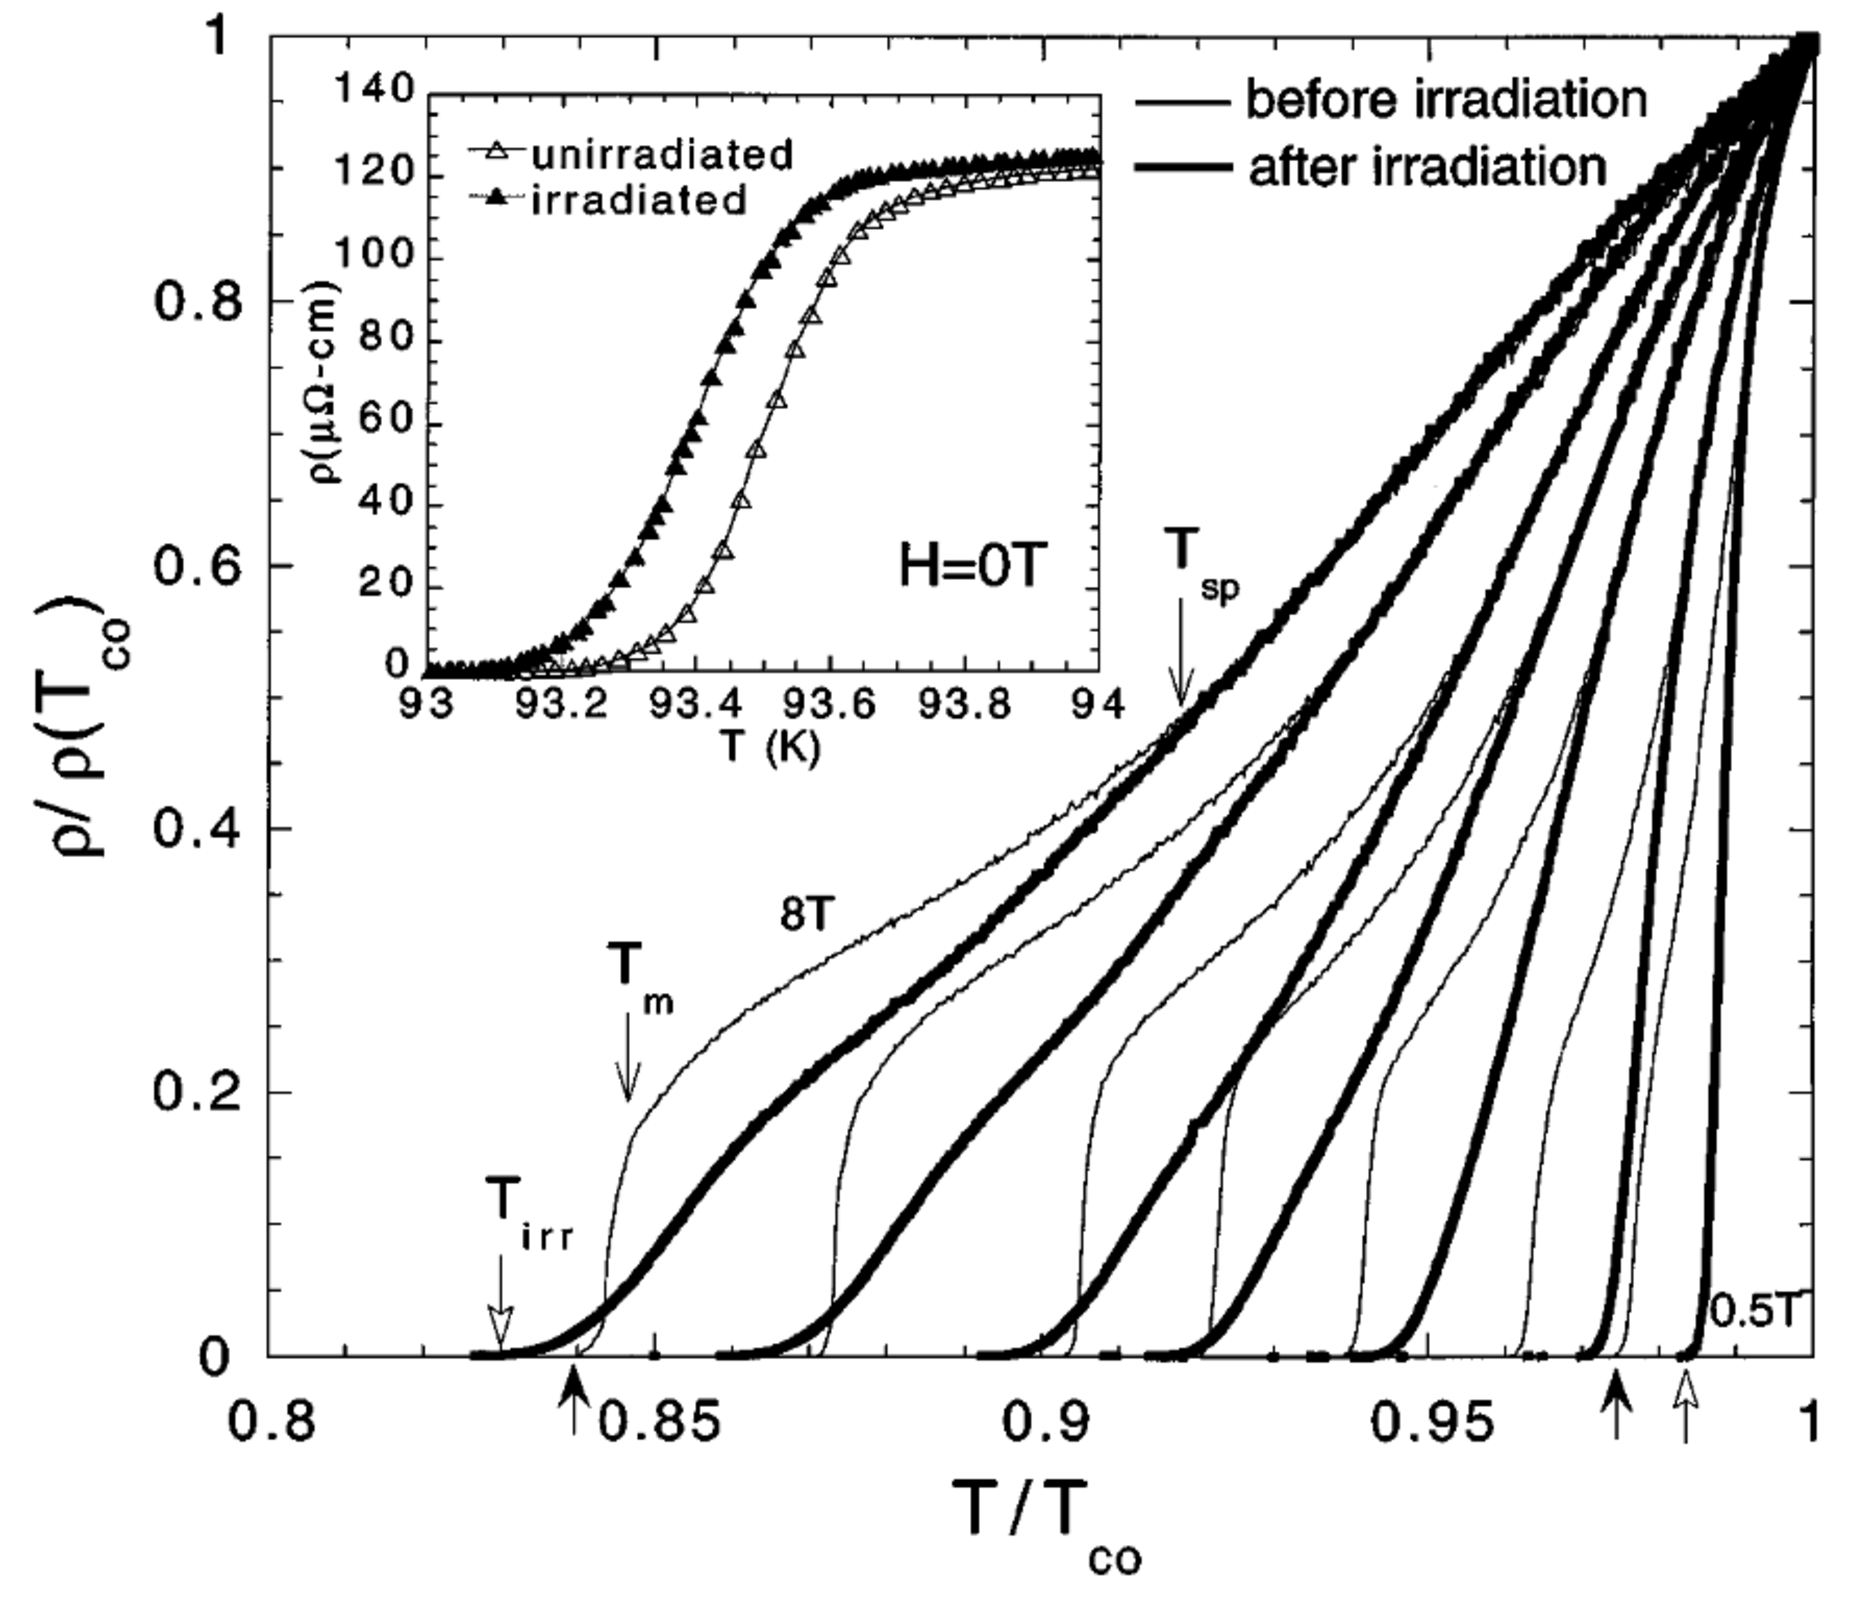
\includegraphics[width=0.42\textwidth]{pre_pos_irradiado}
				\caption{
								Resistividad normalizada en funci\'{o}n de la temperatura para H =
								0,5, 1, 2, 3, 4, 6 y 8 T para el cristal A antes (l\'{i}neas finas)
								y despu\'{e}s (l\'{i}neas gruesas) de la irradiaci\'{o}n con $B_\Phi =
								1.0\,\text{T}$. Las flechas abiertas (post-irradiado) y cerradas
								(pre-irradiado) en el eje de temperatura representan las
								temperaturas de resistividad cero para la curva H = 0.5 T.
								$T_{sp}$ muestra el inicio de la fijaci\'{o}n debido a defectos
								extendidos para H = 8.0 T. El inset muestra la transici\'{o}n de
								campo cero antes y despu\'{e}s de	la irradiaci\'{o}n~\cite{Kwok1998}.
				} 
				\label{fig:pre_pos}
\end{figure}

Kwok \textit{et. al.}~\cite{Kwok1998} hace ver que las l\'{i}neas de
irreversibilidad de los cristales pos-irradiaci\'{o}n cruzan las l\'{i}neas de
irreversibilidad de los cristales pre-irradiados en un campo magn\'{e}tico $H
\sim 2B_\Phi$. La energ\'{i}a de anclaje en el l\'{i}quido de v\'{o}rtice excede
la energ\'{i}a te\'{o}rica de corte de v\'{o}rtice~\cite{Moore1994} en estas
muestras, lo que indica que los defectos columnares extendidos fijan el
l\'{i}quido de manera efectiva debido al enredo topol\'{o}gico. Los autores
determinan la temperatura de inicio del defecto columnar disperso que se fija en
el estado l\'{i}quido, y muestran que la corriente cr\'{i}tica despu\'{e}s de la
irradiaci\'{o}n aumenta a una velocidad mayor con la temperatura decreciente
para el movimiento del v\'{o}rtice perpendicular al plano de separaci\'{o}n que
para el movimiento paralelo al plano de separaci\'{o}n.

En la \figurename~\ref{fig:pre_pos} se puede observar la resistividad
normalizada $\rho/\rho (T_{c0})$ para una muestra, que los autores denominan A,
de cristal antes y despu\'{e}s de la irradiaci\'{o}n, medida con una densidad de
corriente de $0.83\,\text{A/cm}^2$ en un campo magn\'{e}tico. La baja densidad de 
defectos del cristal se evidencia por la marcada ``torcedura'' en la cola de la
transici\'{o}n de preirradiaci\'{o}n hasta $H = 8\,T$. 

\section{Conclusiones}\label{sec:conclusions}

La introducci\'{o}n de defectos columnares creados por irradiaci\'{o}n de monocristales
con iones pesados fue un paso fundamental para demostrar que se pod\'{i}a hacer
crecer en \'{o}rdenes de magnitud la corriente cr\'{i}tica en los SAT, paso esencial
para poder pensar en posibles aplicaciones. Los defectos columnares son defectos
correlacionados en una dimensi\'{o}n, a diferencia de los otros tipos existentes
que lo son puntuales, de dos o tres dimensiones. Antes de realizarse los
experimentos que hemos discutido en este
art\'{i}culo se utilizaban los conceptos tradicionales de anclaje de v\'{o}rtices en
superconductores convencionales para explicar el aumento de corriente cr\'{i}tica:
el v\'{o}rtice, tomado como l\'{i}nea, se ancla dentro del potencial correlacionado. Los
resultados discutidos aqu\'{i} muestran que el rol de los defectos correlacionados
es m\'{a}s importante: ``crean'' las l\'{i}neas y despu\'{e}s las anclan.

Se analizaron las ventajas de tener un arreglo disperso (splay) de defectos
columnares en algunos superconductores de tipo II, as\'{i} como algunas t\'{e}cnicas
para obtener esos arreglos dispersos. Se encontr\'{o} que la dispersi\'{o}n angular en
los defectos columnares posibilita grandes mejoras en las corrientes
persistentes, especialmente en campos y temperaturas altas, y una expansi\'{o}n
sustancial del r\'{e}gimen irreversible.
%
%\section*{Acknowledgment}
%
%The authors would like to thank X. Bertou and H. Asorey for their support  and
%discussion during the preparation of this document.

%\appendix\label{sec:apx}
%
%%\section{Appendix}\label{sec:apx}
%
%As an example, the typical structure of the LAGO acquired data is shown below.
%Two detectors are connected to the input channels 1 and 3, while the channel 2
%has no input. Two triggered pulses are shown. The trigger count (\# c), trigger
%mask and the pulse time stamp (\# t) are included at the end of the 12 temporal
%bins of each pulse. At the end of the second, the FPGA clock frequency (\# x f)
%and the atmospheric pressure and local temperature are also included (\# x s).
%

%\bibliographystyle{JHEP}
%\bibliography{paper_lago_electronics}
\bibliographystyle{IEEEtran}
%\bibliography{IEEEabrv,~/Documents/library, ~/Documents/Mybooks}
\bibliography{IEEEabrv,library,mybooks}
%\bibliography{IEEEabrv,paper_lago_electronics}
%\begin{thebibliography}{1}
%
%\bibitem{AMBAspec}
%ARM, ''AMBA Open Specification´´, webpage. Available
%\url{http://www.arm.com/products/system-ip/amba/amba-open-specifications.php}
%
%\end{thebibliography}

%\IEEEPARstart{T}{his} demo file is intended to serve as a ``starter file''
%for IEEE journal papers produced under \LaTeX\ using
%IEEEtran.cls version 1.8a and later.
%% You must have at least 2 lines in the paragraph with the drop letter
%% (should never be an issue)
%I wish you the best of success.
%
%\hfill mds
% 
%\hfill September 17, 2014

%\subsection{Subsection Heading Here}
%Subsection text here.

% needed in second column of first page if using \IEEEpubid
%\IEEEpubidadjcol

%\subsubsection{Subsubsection Heading Here}
%Subsubsection text here.


% An example of a floating figure using the graphicx package.
% Note that \label must occur AFTER (or within) \caption.
% For figures, \caption should occur after the \includegraphics.
% Note that IEEEtran v1.7 and later has special internal code that
% is designed to preserve the operation of \label within \caption
% even when the captionsoff option is in effect. However, because
% of issues like this, it may be the safest practice to put all your
% \label just after \caption rather than within \caption{}.
%
% Reminder: the "draftcls" or "draftclsnofoot", not "draft", class
% option should be used if it is desired that the figures are to be
% displayed while in draft mode.
%
%\begin{figure}[!t]
%\centering
%\includegraphics[width=2.5in]{myfigure}
% where an .eps filename suffix will be assumed under latex, 
% and a .pdf suffix will be assumed for pdflatex; or what has been declared
% via \DeclareGraphicsExtensions.
%\caption{Simulation results for the network.}
%\label{fig_sim}
%\end{figure}

% Note that IEEE typically puts floats only at the top, even when this
% results in a large percentage of a column being occupied by floats.


% An example of a double column floating figure using two subfigures.
% (The subfig.sty package must be loaded for this to work.)
% The subfigure \label commands are set within each subfloat command,
% and the \label for the overall figure must come after \caption.
% \hfil is used as a separator to get equal spacing.
% Watch out that the combined width of all the subfigures on a 
% line do not exceed the text width or a line break will occur.
%
%\begin{figure*}[!t]
%\centering
%\subfloat[Case I]{\includegraphics[width=2.5in]{box}%
%\label{fig_first_case}}
%\hfil
%\subfloat[Case II]{\includegraphics[width=2.5in]{box}%
%\label{fig_second_case}}
%\caption{Simulation results for the network.}
%\label{fig_sim}
%\end{figure*}
%
% Note that often IEEE papers with subfigures do not employ subfigure
% captions (using the optional argument to \subfloat[]), but instead will
% reference/describe all of them (a), (b), etc., within the main caption.
% Be aware that for subfig.sty to generate the (a), (b), etc., subfigure
% labels, the optional argument to \subfloat must be present. If a
% subcaption is not desired, just leave its contents blank,
% e.g., \subfloat[].


% An example of a floating table. Note that, for IEEE style tables, the
% \caption command should come BEFORE the table and, given that table
% captions serve much like titles, are usually capitalized except for words
% such as a, an, and, as, at, but, by, for, in, nor, of, on, or, the, to
% and up, which are usually not capitalized unless they are the first or
% last word of the caption. Table text will default to \footnotesize as
% IEEE normally uses this smaller font for tables.
% The \label must come after \caption as always.
%
%\begin{table}[!t]
%% increase table row spacing, adjust to taste
%\renewcommand{\arraystretch}{1.3}
% if using array.sty, it might be a good idea to tweak the value of
% \extrarowheight as needed to properly center the text within the cells
%\caption{An Example of a Table}
%\label{table_example}
%\centering
%% Some packages, such as MDW tools, offer better commands for making tables
%% than the plain LaTeX2e tabular which is used here.
%\begin{tabular}{|c||c|}
%\hline
%One & Two\\
%\hline
%Three & Four\\
%\hline
%\end{tabular}
%\end{table}


% Note that the IEEE does not put floats in the very first column
% - or typically anywhere on the first page for that matter. Also,
% in-text middle ("here") positioning is typically not used, but it
% is allowed and encouraged for Computer Society conferences (but
% not Computer Society journals). Most IEEE journals/conferences use
% top floats exclusively. 
% Note that, LaTeX2e, unlike IEEE journals/conferences, places
% footnotes above bottom floats. This can be corrected via the
% \fnbelowfloat command of the stfloats package.


%\section{Conclusion}
%The conclusion goes here.


% if have a single appendix:
%\appendix[Proof of the Zonklar Equations]
% or
%\appendix  % for no appendix heading
% do not use \section anymore after \appendix, only \section*
% is possibly needed

% use appendices with more than one appendix
% then use \section to start each appendix
% you must declare a \section before using any
% \subsection or using \label (\appendices by itself
% starts a section numbered zero.)
%


%\appendices
%\section{Proof of the First Zonklar Equation}
%Appendix one text goes here.
%
%% you can choose not to have a title for an appendix
%% if you want by leaving the argument blank
%\section{}
%Appendix two text goes here.
%
%
%% use section* for acknowledgment
%\section*{Acknowledgment}
%
%
%The authors would like to thank...
%
%
%% Can use something like this to put references on a page
%% by themselves when using endfloat and the captionsoff option.
%\ifCLASSOPTIONcaptionsoff
%  \newpage
%\fi



% trigger a \newpage just before the given reference
% number - used to balance the columns on the last page
% adjust value as needed - may need to be readjusted if
% the document is modified later
%\IEEEtriggeratref{8}
% The "triggered" command can be changed if desired:
%\IEEEtriggercmd{\enlargethispage{-5in}}

% references section

% can use a bibliography generated by BibTeX as a .bbl file
% BibTeX documentation can be easily obtained at:
% http://www.ctan.org/tex-archive/biblio/bibtex/contrib/doc/
% The IEEEtran BibTeX style support page is at:
% http://www.michaelshell.org/tex/ieeetran/bibtex/
%\bibliographystyle{IEEEtran}
% argument is your BibTeX string definitions and bibliography database(s)
%\bibliography{IEEEabrv,../bib/paper}
%
% <OR> manually copy in the resultant .bbl file
% set second argument of \begin to the number of references
% (used to reserve space for the reference number labels box)
%\begin{thebibliography}{1}
%
%\bibitem{IEEEhowto:kopka}
%H.~Kopka and P.~W. Daly, \emph{A Guide to \LaTeX}, 3rd~ed.\hskip 1em plus
%  0.5em minus 0.4em\relax Harlow, England: Addison-Wesley, 1999.
%
%\end{thebibliography}

% biography section
% 
% If you have an EPS/PDF photo (graphicx package needed) extra braces are
% needed around the contents of the optional argument to biography to prevent
% the LaTeX parser from getting confused when it sees the complicated
% \includegraphics command within an optional argument. (You could create
% your own custom macro containing the \includegraphics command to make things
% simpler here.)
%\begin{IEEEbiography}[{\includegraphics[width=1in,height=1.25in,clip,keepaspectratio]{mshell}}]{Michael Shell}
% or if you just want to reserve a space for a photo:

%\begin{IEEEbiography}{M. Sofo Haro}
%Biography text here.
%\end{IEEEbiography}
%
%% if you will not have a photo at all:
%\begin{IEEEbiographynophoto}{H. Arnaldi}
%Biography text here.
%\end{IEEEbiographynophoto}

% insert where needed to balance the two columns on the last page with
% biographies
%\newpage

%\begin{IEEEbiographynophoto}{Jane Doe}
%Biography text here.
%\end{IEEEbiographynophoto}

% You can push biographies down or up by placing
% a \vfill before or after them. The appropriate
% use of \vfill depends on what kind of text is
% on the last page and whether or not the columns
% are being equalized.

%\vfill

% Can be used to pull up biographies so that the bottom of the last one
% is flush with the other column.
%\enlargethispage{-5in}



% that's all folks
\end{document}


